% Sablon pentru realizarea lucrarii de licenta, conform cu recomandarile
% din ghidul de redactare:
% - https://fmi.unibuc.ro/finalizare-studii/
% - https://drive.google.com/file/d/1xj9kZZgTkcKMJkMLRuoYRgLQ1O8CX0mv/view

% Multumiri lui Gabriel Majeri, acest sablon a fost creat pe baza
% codului sursa a lucrarii sale de licenta. 
% Codul sursa: https://github.com/GabrielMajeri/bachelors-thesis
% Website: https://www.gabrielmajeri.ro/
%
% Aceast sablon este licentiat sub Creative Commons Attribution 4.0 International License.

\documentclass[12pt, a4paper]{report}

% Suport pentru diacritice și alte simboluri
\usepackage{fontspec}

% Suport pentru mai multe limbi
\usepackage{polyglossia}

\usepackage{subcaption}
\usepackage{array}

% Setează limba textului la română
\setdefaultlanguage{romanian}
% Am nevoie de engleză pentru rezumat
\setotherlanguages{english}

% Indentează și primul paragraf al fiecărei noi secțiuni
\SetLanguageKeys{romanian}{indentfirst=true}

% Suport pentru diferite stiluri de ghilimele
\usepackage{csquotes}

\DeclareQuoteStyle{romanian}
  {\quotedblbase}
  {\textquotedblright}
  {\guillemotleft}
  {\guillemotright}

% Utilizează biblatex pentru referințe bibliografice
\usepackage[
    maxbibnames=50,
    sorting=none,
]{biblatex}

\addbibresource{bibliography.bib}

% Setează spațiere inter-linie la 1.5
\usepackage{setspace}
\setstretch{1.5}


% Modificarea geometriei paginii
\usepackage{geometry}

% Include funcțiile de grafică
\usepackage{graphicx}
% Încarcă imaginile din directorul `images`
\graphicspath{{./images/}}

% Listări de cod
\usepackage{listings}


% Linkuri interactive în PDF
\usepackage[
    colorlinks,
    linkcolor={black},
    menucolor={black},
    citecolor={black},
    urlcolor={blue}
]{hyperref}

% Simboluri matematice codificate Unicode
\usepackage[warnings-off={mathtools-colon,mathtools-overbracket}]{unicode-math}

% Comenzi matematice
\usepackage{amsmath}
\usepackage{mathtools}

% Pentru captionuri
\usepackage[font=small,labelfont=bf]{caption}

% Formule matematice
\newcommand{\bigO}[1]{\symcal{O}\left(#1\right)}
\DeclarePairedDelimiter\abs{\lvert}{\rvert}

% Suport pentru rezumat în două limbi
% Bazat pe https://tex.stackexchange.com/a/70818
\newenvironment{abstractpage}
  {\cleardoublepage\vspace*{\fill}\thispagestyle{empty}}
  {\vfill\cleardoublepage}
\renewenvironment{abstract}[1]
  {\bigskip\selectlanguage{#1}%
   \begin{center}\bfseries\abstractname\end{center}}
  {\par\bigskip}

% Suport pentru anexe
\usepackage{appendix}

% Stiluri diferite de headere și footere
\usepackage{fancyhdr}

% Metadate
\title{Aplicație de vot digital pentru Consiliul Facultății}
\author{Constantinescu Andrei-Eduard}

% Generează variabilele cu @
\makeatletter

% PENTRU INTRODUCEREA DE COD JS si PYTHON
\newenvironment{code}{\captionsetup{type=figure}}{}
\usepackage{minted,xcolor}
\usemintedstyle{monokai}
\definecolor{bg}{HTML}{282828}

\begin{document}

% Front matter
\cleardoublepage
\let\ps@plain

% Pagina de titlu
\begin{titlepage}

% Redu marginile
\newgeometry{left=2cm,right=2cm,bottom=1cm}

\begin{figure}[!htb]
    \centering
    \begin{minipage}{0.2\textwidth}
        
\includegraphics[width=\linewidth]{logo-ub.png}
    \end{minipage}
    \begin{minipage}{0.5\textwidth}
        \large
        \vspace{0.2cm}
        \begin{center}
            \textbf{UNIVERSITATEA DIN BUCUREȘTI}
        \end{center}
        \vspace{0.3cm}
        \begin{center}
            \textbf{
                FACULTATEA DE \\
                MATEMATICĂ ȘI INFORMATICĂ
            }
        \end{center}
    \end{minipage}
    \begin{minipage}{0.2\textwidth}
        
\includegraphics[width=\linewidth]{logo-fmi.png}
    \end{minipage}
\end{figure}

\begin{center}
\textbf{SPECIALIZAREA INFORMATICĂ}
\end{center}

\vspace{1cm}

\begin{center}
\Large \textbf{Lucrare de licență}
\end{center}

\begin{center}
\huge \textbf{\MakeUppercase{\@title}}
\end{center}

\vspace{3cm}

\begin{center}
\large \textbf{Absolvent \\ \@author}
\end{center}

\vspace{0.25cm}

\begin{center}
\large \textbf{Coordonator științific \\ Lect. dr. Dobrovăț Anca-Mădălina}
\end{center}

\vspace{2cm}

\begin{center}
\Large \textbf{București, iunie 2022}
\end{center}
\end{titlepage}
\restoregeometry
\newgeometry{
    margin=2.5cm
}

\fancypagestyle{main}{
  \fancyhf{}
  \renewcommand\headrulewidth{0pt}
  \fancyhead[C]{}
  \fancyfoot[C]{\thepage}
}

\addtocounter{page}{1}


% Rezumatul
\section*{Rezumat}

Încă din cele mai vechi timpuri, democrația a rămas unul din conceptele cele mai vitale în majoritatea civilizațiilor. Aceasta a ajutat să transforme lumea din jurul oamenilor, dându-le acces la unul dintre cele mai puternice instrumente - votul. În acest sens, oamenii au inventat sisteme din ce în ce mai complexe pentru a gestiona numărul exponențial de oameni chemați să voteze și, mai nou, pentru a rezolva problema unei incertitudini epidemiologice. Astfel, prezenta lucrare de licență vizează implementarea unui de sistem de vot digital pentru Consiliul Facultății.

Scopul aplicației este acela de a oferi membrilor consiliului o modalitate de a-și exprima votul și prin intermediul online-ului, folosind diverse tehnologii moderne de realizare a aplicațiilor web. Printre aceste tehnologii se numără: React, utilizat în dezvoltarea interfeței, Django, folosit în partea de procesare a apelurilor făcute de către interfață și MySQL, pentru gestionarea bazei de date. De asemenea, alături de tehnologiile menționate, au fost folosite librării precum Redux, Chakra UI, React Router și Axios, toate utilizate cu scopul de a eficientiza și a ajuta la o securitate cât mai bună. Rezultatul final este o aplicație ce permite realizarea de procese electorale digitale, astfel încât, în cazul unei noi situații epidemiologice nefavorabile, Consiliul Facultății să își poată continua activitatea cât mai eficace.

\newpage

\section*{Abstract}

Democracy has been one of the most lasting ways in which civilizations have been organized through history. It helped transform the world, as the leadership was centered around the people by giving them access to one of the most powerful tools - the vote. As a consequence, one has invented increasingly complex voting systems capable to manage the exponential increase in the number of people called to vote and, more recently, to solve the problem of epidemiological uncertainty. Thus the objective of the current bachelor's thesis is to develop and implement a digital voting system for the Faculty Council.

The application aims to provide the Faculty’s Board members with a way to express their vote online, using a variety of modern web application technologies, among which: React, used in the development of the interface, Django, used in the part processing of calls made by the interface and MySQL, for database management. Along the above-mentioned technologies, there were used libraries such as Redux, Chakra UI, React Router and Axios, in order to increase effectiveness and security. The end result is an application that allows the realization of digital electoral processes, so that, in case of a new pandemic, the Faculty Council can continue its activity as effectively as possible.


\tableofcontents
\listoffigures

% Main matter
\cleardoublepage
\pagestyle{main}
\let\ps@plain\ps@main

\addcontentsline{toc}{section}{\protect\numberline{}Introducere}%
\section*{Introducere}

Trăim în era în care tehnologia a devenit parte din rutina noastră zilnică și, conform unui studiu afiliat cu Universitatea din California \cite{online_vs_offline_communication}, am ajuns să comunicăm mai mult în online decât față în față. Acest fapt a jucat un rol important în timpul pandemiei de Covid-19, când, datorită faptului că populația generală a fost supusă unor restricții ce limita, temporar, interacțiunea socială, oamenii au reușit să se adapteze noului stil de viață și, de asemenea, comunicării în online. Multe dintre activitățile ce se desfășurau față în față au fost nevoite să fie trecute în format digital. De la o simplă oră de curs în cadrul facultății, până la un job full-time, oamenii au fost nevoiți să găsească mijloace pentru a putea continua să își desfășoare aceste activități.

Printre entitățile afectate de pandemia de Covid-19, se numără, în mare parte, și cele care erau nevoite să își consolideze direcțiile decizionale printr-un vot al membrilor acestora. Ele au fost constrânse să își mute ședințele într-un format digital și, implicit, toate procesele electorale realizate. Acest fapt a adus o schimbare în modul în care erau stabilite hotărârile, de la modul clasic - fizic, la un simplu chestionar, în online. În acest fapt, aplicația vizează implementarea unei platforme digitale de vot ce are ca scop principal eficientizarea realizării proceselor electorale în cadrul Consiliului Facultății.

În următoarele capitole se va prezenta, atât soluția propusă pentru o astfel de platformă, cât și tehnologiile folosite și procesul de implementarea a acestora. Primul capitol are un rol introductiv, în care vor fi detaliate concepte din arhitectura aplicației. Al doilea capitol va prezentarea implementarea conceptelor teoretice, iar ultimul capitol se va referi la utilizarea aplicației, atât din punctul de vedere al unui utilizator, cât și al unui administrator.

\chapter{Arhitectura aplicației}

\section{Aplicațiile web}

\subsection{Scurt istoric}

Primele aplicații web au apărut la începutul anului 1990 \cite{history_of_js} și, dat fiind că era o tehnologie nouă, acestea nu erau nimic mai mult decât pagini statice, pline cu text, urmând ulterior să fie îmbibate cu elemente grafice - imagini, videoclipuri, audio. Anul 1995 a avut o însemnătate deosebită pentru îmbunătățirea acestor site-uri: inventarea limbajului JavaScript de către Brandan Eich \cite{brandan_eich_js}, pe când era inginer la Netscape Communications Corporation. Acest limbaj de programare rulează în browser, pe partea de client, și este nelipsit din ceea ce înseamnă web, având în vedere că, în 2019, aproximativ 95\% \cite{popularity_of_js} din aplicațiile web de atunci rulau JavaScript. Importanța datorată acestui limbaj de programare este dată de începerea trecerii de la pagini statice la pagini dinamice, ce reacționează în funcție de acțiunile realizate de către utilizator, permițând, astfel, o multitudine de noi posibilități în materie de "user experience". Această trecere a marcat un nou început pentru aplicațiile web moderne.


\subsection{Importanța aplicațiilor web}

Folosim aplicații web zi de zi pentru tot felul de activități, de la aplicații de divertisment precum Netflix și YouTube până la magazine online sau chiar platforme de social media. Putem spune, astfel, că marea majoritate a activității noastre din online este realizată pe aplicații web. Pe lângă aplicațiile publice, destinate oricui, există și aplicații web private, folosite de un anumit grup de oameni, de cele mai multe ori în contextul locului de muncă, fiind deseori protejate de mai multe straturi de securitate și au ca scop, ori administrarea aplicațiilor publice, ori organizarea internă sau gestionarea de informații în cadrul grupului.

\section{Structura aplicației}

Voting App este alcătuită din trei componente de bază într-o aplicație web:

\begin{itemize}
    \item Componenta de interfață (frontend), realizată în JavaScript și React, ce reprezintă partea interactivă a aplicației
    \item Componenta de gestionare a apelurilor făcute de către interfață (backend), bazată pe Python în cadrul framework-ului Django. Această componentă are ca rol punerea în funcțiune a unor operații ce pot fi realizate în interfață, astfel încât acestea să fie procesate și, în funcție de nevoie, salvate în baza de date.
    \item Componenta ce gestionează baza de date, realizată cu ajutorul SQL și al sistemului de management MySQL.
\end{itemize}

\subsection{Structura aplicației client}

Aplicația client reprezintă interfața cu care utilizatorul interacționează, aceasta fiind construită utilizând librăria React pentru JavaScript. Deși nu este un framework integral, precum Angular sau Vue, React rămâne în continuare una dintre opțiunile principale atunci când este vorba de dezvoltarea unei aplicații web. Popularitatea acestei librării este dată de așa-zisele componente reutilizabile ce pot fi folosite ori de câte ori este nevoie, oriunde, în aplicație, eliminând astfel necesitatea rescrierii de cod, ajutând la realizarea unuia dintre principiile dezvoltării software - DRY (\enquote{Don't Repeat Yourself}) \cite{DRY_book}.

Componentele, ce reprezintă piesa centrală a librăriei React, nu sunt nimic mai mult decât funcții de JavaScript ce returnează elemente de tip JSX. Aceste elemente sunt o combinație între JavaScript și HTML astfel încât să fie utilizate toate conceptele unui limbaj de programare (variabile, funcții, loop-uri, iteratoare, etc.) în tag-uri HTML generate atât static, cât și dinamic. În Voting App, există o singură componentă principală (App.js) ce face legătura cu toate celelalte componente, fiind alcătuită din toate rutele aplicației. Aceste rute sunt componente de tip \enquote{Route} ce reprezintă paginile pe care le poate accesa utilizatorul aplicației. Tot în această componentă principală este realizată și logica ce determină paginile disponibile unui utilizator, în funcție de rolul pe care îl deține. Un utilizator cu rolul de administrator va avea acces la pagini ce țin de controlul aplicației și ce oferă puteri sporite asupra acesteia. Principalele pagini la care un simplu utilizator are acces sunt cele de vizualizare a datelor și cele în care este nevoit să își exprime votul sau în care este nevoit să introducă date personale.

De asemenea, pentru a menține un aspect simplist și modern, am folosit librăria Chakra UI. Aceasta dispune de o varietate de componente prestabilite și de un sistem modular pentru a defini propriile componente stilistice. Pentru a utiliza această librărie, componenta principală \enquote{App.js} a fost pusă în interiorul componentei \enquote{ChakraProvider} pentru a avea acces la toate elementele librăriei.

În continuare, pentru a accesa endpoint-urile din aplicația de backend și, implicit, pentru a procesa datele primite, am folosit librăria Axios, ce are a scop simplificarea modului de lucru cu request-uri și procesarea datelor primite și trimise. Aceasta are la bază transmiterea datelor sub forma JSON (JavaScript Object Notation) \cite{JSON_what_is}, reprezentând un mod foarte ușor de lucru, în special în aplicația client, dat fiind că JavaScript lucrează implicit cu JSON-uri.

\begin{figure}[!h]
    \centering
    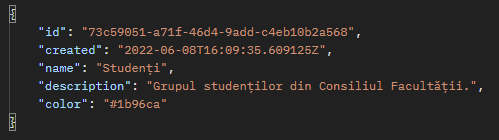
\includegraphics[width=115mm]{images/json_example.png}
    \caption{Exemplu de JSON folosit în aplicație}
\end{figure}

Nu în ultimul rând, pentru a menține \enquote{state-ul} în întregimea aplicației, am folosit librăria Redux. Aceasta este utilizată pentru a accesa și a modifica variabile necesare pe tot parcursul folosirii aplicației, precum starea autentificat / neautentificat sau datele utilizatorului (id, nume, prenume, etc.). Asemănător cu Chakra UI, pentru funcționarea librăriei a fost necesară punerea componentei principale întru-un provider customizabil, unde sunt declarate toate operațiile. 

\subsection{Structura aplicației server}

Aplicația server este realizată în limbajul Python, fiind folosit framework-ul Django, alături de librăria Django REST Framework ce permite utilizarea conceptelor de REST API în aplicație. Aplicația de backend este structurată de următoarele elemente importante pentru a funcționa eficient:

\begin{itemize}
    \item \enquote{Model}: definește reprezentarea schematică și structura unui obiect din baza de date, alături de legăturile pe care acesta le are cu alte obiecte.
    \item \enquote{Url}: reprezintă rutele unde se pot face cereri HTTP și face legătura dintre funcțiile aplicației și exterior.
    \item \enquote{View}: conține funcțiile apelate de către Url atunci când este accesată o rută și întoarce un răspuns HTTP.
    \item \enquote{Serializer}: transformă un model definit în Python în format JSON pentru a putea fi transmis mai departe de către View.
\end{itemize}

Framework-ul Django funcționează, în mare, pe modelul MVC (\enquote{Model View Controller}) \cite{MVC_what_is} și are la bază o multitudine de funcționalități, în special pe partea de View-uri. Aici sunt definite metodele și tipurile acestora (get, post, delete, etc.) și se împart în două categorii:

\begin{itemize}
    \item Metode aparținând unui \enquote{View Set}. View Set-ul este o clasă ce grupează mai multe metode pentru definirea rapidă a operațiilor de tip CRUD (\enquote{Create, Read, Update, Delete}) pentru un singur model.
    \item Metode de sine stătătoare. Metode ce sunt definite în afara View Set-urilor și au nevoie de o adnotare care să permită framework-ului să înțeleagă ce fel de cerere este făcută prin acea metodă, ca de exemplu: @GET, @PUT, @DELETE, etc..
\end{itemize}

De asemenea, pentru îndeplinirea unor funcționalități din interfața Voting App, a fost necesară trimiterea de email-uri. Pentru a realiza acest lucru eficient a fost folosit conceptul de multithreading. Astfel, atunci când era cerută trimiterea unui mail, aplicația de backend crea un nou fir de execuție pentru a o procesa, putând, astfel, gestiona în continuare alte cereri.

\subsection{Baza de date}

Pentru a salva datele procesate de către aplicația server, am folosit o bază de date MySQL. Legătura dintre MySQL și Django a fost realizată utilizând funcționalitatea integrată în framework. De asemenea, în baza de date au fost folosite și alte tabele în afară de cele pentru modelele definite precum:

\begin{itemize}
    \item \enquote{django\_rest\_passwordreset}, utilizat pentru a salva date necesare procesului de resetare a parolei de către utilizator.
    \item \enquote{django\_migrations}, folosit pentru a memora date despre migrațiile făcute în baza de date.
\end{itemize}

\begin{figure}[!h]
    \centering
    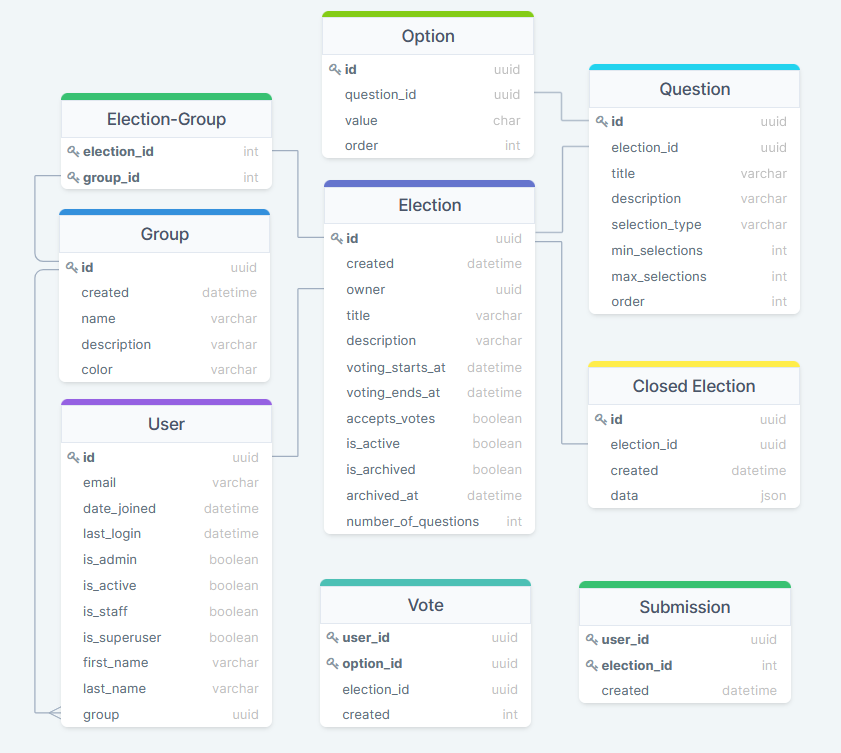
\includegraphics[width=135mm]{images/db_example.png}
    \caption{Diagrama structurii și relațiilor modelelor din baza de date}
\end{figure}

\chapter{Implementarea aplicației}

\section{Tehnologii folosite pentru aplicația client}

\subsection{JavaScript}

JavaScript este un limbaj de programare ce permite realizarea de funcționalități complexe pentru paginile web. A fost lansat în 1995 sub numele de LiveScript \cite{brandan_eich_js} și și-a făcut un renume, fiind, în 2021, cel mai popular limbaj de programare, conform unui chestionar realizat de către Stack Overflow \cite{js_stackoverflow}. Reușita JavaScript-ului vine atât din eficiența prin care reușește să dinamizeze paginile web, dar și prin ecosistemul de librării create în jurul său. Librăriile bazate pe JavaScript sunt în continuă dezvoltare și creștere, astăzi existând mai mult de un milion de librării listate oficial \cite{number_of_js_libraries}.

\subsection{React}

Așa și cum apare pe pagina oficială, React nu este nimic mai mult decât o librărie pentru realizarea interfețelor \cite{react_webpage}. A fost creat de către Jordan Walke, un inginer al companiei Facebook, în 2011 și implementat în newsfeed-ul platformei în același an, urmând ca, mai târziu, când Facebook a achiziționat Instagram, să fie implementat și acolo. Cu timpul, React s-a dezvoltat, iar, în 2013, a devenit open source, fapt ce a dus la o dezvoltare exponențială în materie de capabilități și funcționalități pe care le poate realiza. Astăzi, React este cea mai populară soluție pentru interfața unei aplicații web \cite{popularity_of_react}.

\newpage

\begin{figure}[!ht]
    \centering
    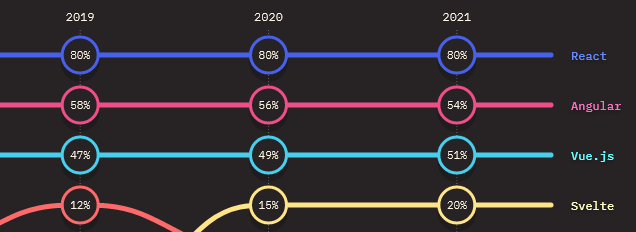
\includegraphics[width=135mm]{images/react_popularity.png}
    \caption{Clasament \enquote{State of JavaScript} pentru librăriile de frontend, după utilizare}
\end{figure}


Eficiența librăriei este realizată de un cumul de factori precum:

\begin{itemize}
    \item Componente reutilizabile. Aceste componente reprezintă unul din cele mai importante concepte în React, permițând reutilizarea acestora oriunde în aplicație. Ele pot fi customizate ușor, dat fiind că acceptă parametrii când vine vorba de procesat starea internă și de afișat informații.
    
    \item DOM Virtual. Pentru a eficientiza schimbările rapide pe care le realizează librăria, React are implementat un DOM virtual, adică o copie mai \enquote{lightweight} a DOM-ului real. Operațiile de schimbare ale DOM-ului real sunt lente, astfel, React poate updata numai componentele care sunt alternate, neavând nevoia de a redesena tot DOM-ul.
    
    \item Curs de date unidirecțional. React urmează un curs de date unidirecțional, astfel, când este dezvoltată o aplicație React, deseori componentele sunt așezate într-un mod \enquote{parent-child}, astfel informația trecând de la componenta părinte la componenta copil într-un mod direct.
    
    \item Tool-uri dedicate pentru debugging. Facebook a lansat o extensie open source pentru browser ce are ca scop principal inspectarea componentelor React și a ierarhiei acestora direct din browser.
    
\end{itemize}

Astfel, am folosit toți acești factori în realizarea aplicației Voting App, începând de la cele mai mari componente (componenta \enquote{Route}) până la cele mai mici (butoane, texte, inputuri, etc.).

\subsection{NPM}

Node Packet Manager (NPM) reprezintă, în același timp, 2 concepte diferite. În primul rând este cel mai mare registru online pentru publicarea pachetelor open source realizate în Node.js și, în al doilea rând, este un modul ce suplimentează linia de comandă cu mai multe instrucțiuni, astfel încât să fie posibilă interacțiunea cu registrul online pentru ajutarea, atât în instalarea pachetelor necesare unui proiect, cât și pentru gestionarea versiunii și dependențelor pachetelor \cite{what_is_npm}.

Pentru a folosi React, este necesară o multitudine de pachete ce trebuie instalate cu ajutorul NPM. Aceste pachete sunt salvate în directorul \enquote{node\_modules}, iar versiunea lor în fișierul \enquote{package{.}json} sub tag-ul \enquote{dependencies}. Instalarea pachetelor s-a efectuat utilizând comanda \enquote{npm install nume\_pachet}.

\subsection{Axios}

Axios este o simplă librărie de JavaScript ce ajută la realizarea request-urilor HTTP de pe client \cite{axios_docs}. Librăria este bazată pe conceptul de \enquote{Promisiune}. O promisiune reprezintă o eventuală completare sau un eventual eșec al unei operații asincrone și a valorii returnate de către aceasta \cite{what_is_promise}.

În Voting App am folosit o instanță definită pentru client, astfel încât adresa IP la care sunt făcute request-urile către aplicația backend să fie modificată ușor.

\begin{code}
\begin{minted}[bgcolor=bg,frame=lines,framesep=2mm,fontsize=\footnotesize,baselinestretch=1]{js}
export default axios.create({
    baseURL: 'http://127.0.0.1:8000',
    headers: {
        "Content-type": "application/json"
    }
});
\end{minted}
\captionof{figure}{Clientul Axios pentru Voting App}
\label{code:axios-code}
\end{code}
\hfill

De asemenea, pentru a putea oferi aplicației de backend o modalitate de a identifica persoana de unde a fost făcut un request, se va trimite, pe lângă datele request-ului, și un token. Acest token este trimis în header-ul request-ului și este primit de către utilizator atunci când este făcută autentificarea. În funcție de acest token, serverul poate identifica dacă un utilizator are rol de admin sau nu și poate bloca un request făcut pe o cale protejată dacă utilizatorul nu îndeplinește acest criteriu.

Pentru a putea realiza diferența dintre tipurile de răspunsuri primite atunci când este făcut un request, aplicația de backend va trimite și un cod HTTP. Aceste coduri se împart în următoarele categorii \cite{http_codes}:

\begin{itemize}
    \item Răspunsuri informative (100–199)
    \item Răspunsuri de succes (200–299)
    \item Mesaje de redirecționare (300–399)
    \item Erori de client (400–499)
    \item Erori de server (500–599)
\end{itemize}

În funcție de codul primit, aplicația de frontend observă dacă request-ul făcut a avut succes sau nu și va reacționa ca atare.

\subsection{Redux}

Redux este o librărie de JavaScript menită să gestioneze state-ul în aplicație. A fost creat în 2015 de către Dan Abramov și Andrew Clark și este cea mai des folosită librărie pentru acest lucru. Modul în care funcționează Redux este unul relativ simplu. Este creat un \enquote{store} central în care este ținut intregul state al aplicației. Fiecare componentă poate accesa acest \enquote{store} fără a avea nevoie de informații suplimentare, funcționând asemănător unor variabile globale \cite{redux_docs}. Există trei componente principale ce formează Redux, și anume:

\begin{itemize}
    \item Actions, reprezintă event-uri ce pot modifica state-ul. Ele sunt singura modalitate prin care se pot trimite date către \enquote{store} în cadrul unei metode \enquote{dispatch}. Există mai multe tipuri de acțiuni și, de aceea, ele sunt nevoite să conțină o proprietate \enquote{type}.
    \item Reducers, funcții ce iau state-ul curent al aplicației, aplică o acțiune și întorc tot un state. Ele sunt folosite pentru gestionarea continua a variabilelor ce se pot modifica pe parcursul utilizării aplicației.
    \item Store, fiind obiectul central în care sunt salvate datele. Pentru ca o componentă să aibă acces la acestea, aplicația a fost pusă într-un provider în care au fost definite stările inițiale.

\end{itemize}

În cadrul Voting App am folosit Redux pentru a gestiona două state-uri diferite. Primul state conține date despre autentificare - dacă există un utilizator autentificat pe platformă și token-ul pe care acesta l-a primit din aplicația de backend atunci când a fost făcută autentificarea. Al doilea state pe care Redux l-a gestionat în Voting App este cel al utilizatorului autentificat, în care sunt salvate date precum: identificatorul utilizatorului, numele și prenumele acestuia, adresa de email, grupul din care face parte și nu numai. De asemenea, în cadrul aplicației au fost definite acțiuni care vizează login-ul și logout-ul de pe platformă și schimbarea datelor personale.

\subsection{Chakra UI}

O aplicație modernă are nevoie și de o stilizare ca atare și consistentă. Pentru a îmbunătății acest proces și pentru a oferi utilizatorului o experiență cât mai intuitivă pe platformă a fost folosită librăria Chakra UI. Această librărie permite dezvoltatorilor utilizarea unor componente deja stilizate și posibilitatea de a stiliza propriile componente într-un mod foarte rapid și eficient din punct de vedere al timpului necesar. Unul dintre principalele avantaje ale Chakra UI față de alte librării de stilizare este modul în care elementele reacționează la diferite rezoluții și ecrane (de la mobil și tabletă până la desktop), fiind o librărie \enquote{responsive}. A fost realizată de către Segun Adebayo și are peste 26 de mii de star-uri pe GitHub \cite{chakra_github}. Un alt avantaj al acestei librării este dat de ușurința cu care poate fi realizată o temă proprie - este suficientă doar descrierea unui obiect în care sunt puse culorile și măsurătorile dorite, librăria dispunând și de o implementare ușoară a unui \enquote{dark theme}.

Pentru a accesa componentele dispuse de către Chakra UI, este necesară punerea aplicației într-un provider numit \enquote{ChakraProvider}, asemenea provider-ului librăriei Redux. În Voting App, toate componentele sunt stilizate utilizând proprietăți ale librăriei, ca de exemplu: \enquote{mr} pentru a seta marginea la dreapta a unei componente sau \enquote{borderRadius} pentru a curba marginea unui element.

De asemenea, au fost folosite componente prestabilite, în special pentru input-urile din formulare, deoarece librăria dispune de un ecosistem bine definit pentru ceea ce înseamna \enquote{user feedback} atunci când vine vorba de validare.

Meniul principal al Voting App este realizat utilizând un Flexbox \cite{flexbox}, iar cartonașele ce reprezintă buletinele de vot conțin Box-uri stilizate pentru a oferi un efect de umbră. În același sens, la baza fiecărei pagini se află un layout de standard. Acest layout este alcătuit din:

\begin{itemize}
    \item Navbar. Reprezintă partea de sus a layout-ului și conține, pentru desktop, doar un buton cu numele utilizatorului astfel ca, atunci când este apăsat, să deschidă un meniu cu două opțiuni: pagina de setări și deconectare. Pentru mobil, această componentă afișează un al doilea buton, de tip \enquote{burger}, care deschide utilizatorului Sidebar-ul (acesta fiind ascuns din start pe mobil).
    \item Sidebar. Conține toate rutele de bază pe care utilizatorul le poate accesa pentru a vizualiza și a prelucra date în cadrul aplicației (pagina principală, pagina cu toate voturile disponibile, pagina cu toate grupurile active și dashboard-ul pentru administrator, în cazul în care utilizatorul are acest rol). Pentru mobil, acesta este ascuns și trebuie deschis prin apăsarea butonului din Navbar. De asemenea, atunci când utilizatorul se află pe mobil, Sidebar-ul dispune de un buton suplimentar pentru închiderea sa.
    \item Titlebar. Este alcătuit din două elemente - numele paginii curente și un buton care redirecționează utilizatorul cu un pas înapoi pe aplicație.
    \item Footer. Conține două link-uri care duc la pagina principală a site-ului facultății și la pagina oficială de contact al secretariatului facultății.
\end{itemize}

\hfill

\begin{figure}[!h]
    \centering
    
\includegraphics[width=135mm]{images/navbar_desktop.png}
    \caption{Navbar pe desktop. În stânga, fiind începutul Sidebar-ului}
\end{figure}

\begin{figure}[!h]
    \centering
    
\includegraphics[width=115mm]{images/navbar_mobil.png}
    \caption{Navbar pe mobil, cu butonul \enquote{burger}}
\end{figure}


\section{Tehnologii folosite pentru aplicația server}

\subsection{Python}

Python este un limbaj de programare interpretat, orientat pe obiecte, ce excelează prin lizibilitatea codului și versatilitate. A fost creat de către Guido Van Rossum, iar prima versiune oficială a fost lansată în anul 1994. Încă de atunci a fost supus unor schimbări și îmbunătățiri constante, dat fiind că în anul 2000 a fost lansată versiunea 2.0 a limbajului, iar, mai recent, în 2008, versiunea 3.0. Conform unei statistici independente \cite{popularity_of_python}, Python ocupa, în sfertul al patrulea al anului 2021, poziția întâi în numărul de apariții în repository-urile de pe GitHub, acest fapt dovedind popularitatea limbajului.

\begin{figure}[!h]
    \centering
    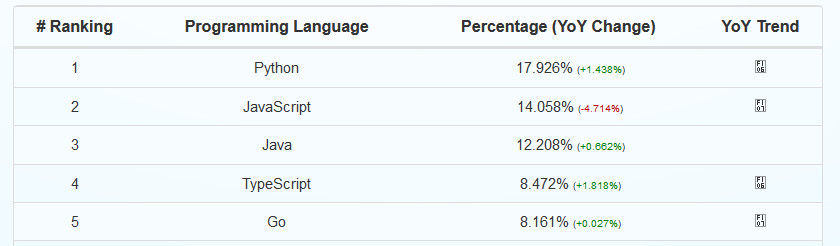
\includegraphics[width=140mm]{images/python_popularity.png}
    \caption{Popularitatea limbajelor de programare pe GitHub}
\end{figure}

Față de alte limbaje de programare precum C și C++, unde este necesară compilarea codului pentru a putea fi executat, adică traducerea codului scris în limbaj mașină ce poate fi executat direct pe CPU, Python funcționează împreună cu un interpretor. Acest interpretor preia codul scris și îl transformă în bytecode, astfel încât să poată fi rulat de către acesta. Această abordare vine cu un set de avantaje, printre care se numără:

\begin{itemize}
    \item Portabilitate. Atunci când un program este scris într-un limbaj ce necesită compilare, acest proces devine specific pentru device-ul pe care este executat compilatorul. În schimb, interpretorul funcționează în același mod pe toate sistemele de operare, astfel, nu există diferențe între un cod scris în Windows, față de un cod scris în Linux.
    \item Scriere dinamică. Implementarea \enquote{dynamic typing-ului} într-un limbaj compilat este foarte grea și poate duce la generarea multor erori. Totuși, pentru un limbaj interpretat, \enquote{dynamic typing-ul} este implementat de la sine, astfel dezvoltatorii putând să evite declararea tipului unei variabile (int, string, etc.).
    \item Debugging mai rapid. Interpretorul rulează programul linie cu linie și, atunci când întâmpină o eroare, dezvoltatorul știe concret cauza și linia la care a apărut.
\end{itemize}

Pentru Voting App a fost folosită versiunea de Python 3.10.1.

\subsection{Django}

Django este un framework open source pentru backend realizat în Python ce permite dezvoltarea de aplicații web rapid și scalabil. Framework-ul a fost conceput începând cu anul 2003, iar, în 2005 a devenit open source. Încă de atunci, a avut parte de o continuă dezvoltare, atingând, în 2008 versiunea 1.0, iar, în 2022, versiunea 4.0. Unul dintre avantajele Django este simplitatea dezvoltării aplicațiilor, urmând o structură MVC (\enquote{Model, View, Controller}) \cite{MVC_what_is}.

\begin{figure}[!h]
    \centering
    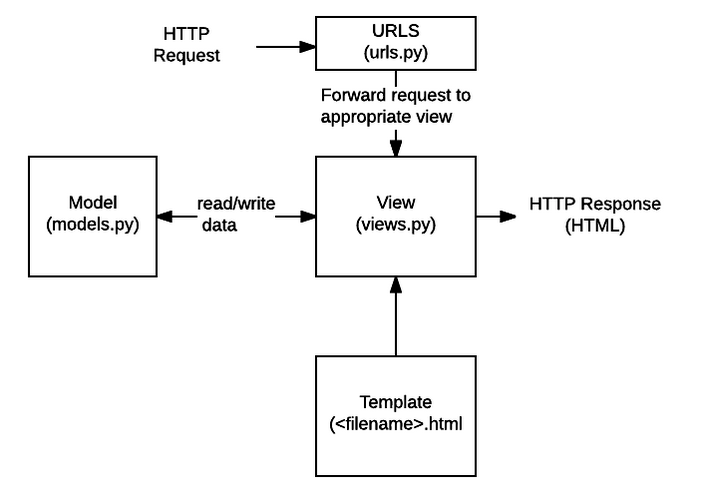
\includegraphics[width=130mm]{images/django.png}
    \caption{Arhitectura framework-ului Django}
\end{figure}

Scopul utilizării Django în Voting App a fost folosirea librăriei Django REST Framework, ce permite utilizarea lui drept un serviciu de API. API (\enquote{Application Programming Interface}) este un mecanism ce permite comunicarea între două componente software utilizând un set de reguli, definiții și protocoale. Arhitectura acestui mecanism este împărțită în client și server - clientul trimite request-uri către server, așteptând un răspuns. Există mai multe tipuri de API, iar cel folosit de Voting App este REST API.

REST (\enquote{Representational State Transfer}) definește un set de operații precum GET, PUT, DELETE, POST, etc. pe care un client le poate accesa pentru a comunica date printr-un protocol HTTP. Cea mai importantă caracteristică a REST este lipsa unei \enquote{stări}, adică serverul nu salvează datele transmise între request-uri. \cite{what_is_rest}. Datele transmise de un REST API sunt de tip text, lipsite de orice elemente grafice sau audio.

\begin{figure}[!h]
    \centering
    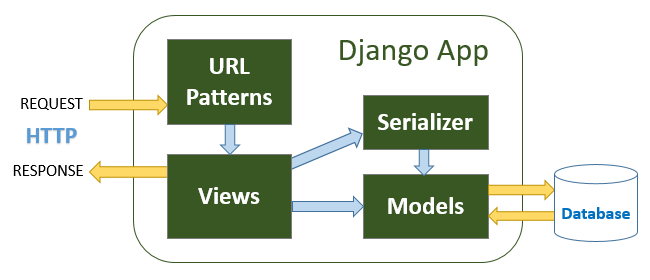
\includegraphics[width=110mm]{images/rest_flow.png}
    \caption{Modul de funcționare al Django REST Framework}
\end{figure}

Aplicația Voting App implementează toate conceptele de baze ale Django REST Framework. În primul rând au fost create modelele necesare pentru a susține un proces electoral:

\begin{itemize}
    \item User. Reprezintă clasa de bază a unui utilizator și conține datele acestuia - identificator, nume, prenume, email și grupul din care face parte. De asemenea, pe lângă aceste date, modelul User conține și structuri tip \enquote{boolean} pentru salvarea informațiilor cu vedere la rolurile pe care acesta le are - \enquote{admin}, \enquote{staff} sau \enquote{superuser}.
    \item Group. Acest model are la bază câmpuri pentru identificator, nume, descriere și culoare. Mai mulți utilizatori fac parte dintr-un grup, iar un singur utilizator nu poate face parte din două sau mai multe grupuri în același timp.
    \item Election. Este cea mai complexă clasă din Voting App, dat fiind necesitatea creării unui sistem cât mai customizabil și flexibil de votare. Acesta are câmpuri pentru \enquote{owner}, titlu, descriere, data începerii votului, data încheierii votului, data la care acesta a fost arhivat și variabile de tip \enquote{boolean} pentru a menține starea - \enquote{is\_active} și \enquote{is\_archived}. De asemenea mai are două câmpuri variabile, unul în care memorează numărul de întrebări din buletinul de vot și unul în care memorează grupurile de utilizatori care iau parte la procesul electoral.
    \item Question. Reprezintă o întrebare pusă într-un buletin de vot, aceasta putând apărea într-un număr aproape nelimitat pentru un singur proces electoral. Conține câmpuri pentru titlu, descriere și, în funcție de tipul întrebării (\enquote{single choice} sau \enquote{multiple choice}) schimbă valorile de opțiuni minime și maxime pe care un participant la vot le poate selecta.
    \item Option. Conține valoarea unei opțiuni din cadrul unei întrebări.
    \item Vote. Asemenea unei ștampile puse pe un buletin de vot, clasa Vote conține date despre opțiunea aleasă la o întrebare de către utilizator și procesul electoral la care acesta a luat parte.
    \item Submission. Pentru a putea vedea ce utilizatori au votat sau nu, clasa Submission funcționează drept un registru în care sunt adăugate date atunci când utilizatorul și-a exprimat votul. Această clasă nu memorează opțiunile alese de către utilizator, ci doar dacă acesta a votat sau nu la un anumit proces electoral.
\end{itemize}

De asemenea, pentru a arhiva un proces electoral încheiat, a fost realizat modelul \enquote{ClosedElection} cu scopul de a salva o copie a datelor finale pentru a le putea arhiva și pentru a putea fi mai ușor de accesat mai târziu. Acesta conține o referință la procesul inițial și un câmp JSON în care sunt salvate toate datele aferente.

În al doilea rând, Voting App se folosește de serializatoare pentru a transforma datele în format JSON astfel încât să fie transmise unui request. Aceste serializatoare au fost realizate pentru toate modelele declarate.

\begin{code}
\begin{minted}[bgcolor=bg,frame=lines,framesep=2mm,fontsize=\footnotesize,baselinestretch=1]{python}
class UserSerializer(serializers.ModelSerializer):
    group = GroupSerializer(many=False, read_only=True)
    class Meta:
        model = User
        fields = ['id', 'email', 'first_name', 'last_name', 'group', 'date_joined', \
            'last_login', 'is_staff', 'is_active']
\end{minted}
\captionof{figure}{Exemplu de serializator pentru modelul User}
\label{code:serializer-code}
\end{code}
\hfill

Avantajele folosirii serializatoarelor integrate în Django REST Framework este acela că permit un mod de utilizare foarte modular, dezvoltatorul putând să decidă ce câmpuri să includă sau să excludă.

\hfill

Nu în ultimul rând, pentru a putea lucra cu modelele și serializatoarele create, au fost implementate \enquote{View-uri}. Acestea au rolul de a procesa request-ul primit printr-o rută, adică, în Django, printr-un Url. Url-urile nu sunt nimic mai mult decât declarații ale rutelor prin care un client poate apela API-ul și, în funcție de request-ul făcut, execută View-ul atribuit. Url-urile pot primi un număr nedefinit de parametrii. Pentru Voting App, cele mai multe rute au primit ca parametru identificatorul obiectului pe care clientul dorește să îl acceseze

\begin{code}
\begin{minted}[bgcolor=bg,frame=lines,framesep=2mm,fontsize=\footnotesize,baselinestretch=1]{python}
    path('elections/<str:pk>/submit/', views.submitVotes),
    path('elections/<str:pk>/submissions/', views.getElectionSubmissions),
    path('elections/active/', views.getActiveElections),
    path('elections/inactive/', views.getInactiveElections),
    path('elections/<str:pk>/groups/', views.getGroupsFromElection),
    path('elections/<str:pk>/close/', views.closeElection),
\end{minted}
\captionof{figure}{Exemplu de Url-uri pentru modelul Election}
\label{code:url-code}
\end{code}
\hfill

În Voting App au fost folosite două tipuri de View-uri: de sine stătătoare și \enquote{ViewSet-uri}. View-urile de sine stătătoare sunt funcții ce nu aparțin unei clase și în care dezvoltatorul trebuie să specifice tipul request-ului (GET, POST, etc.) prin adnotarea \enquote{@api\_view}. De asemenea, pentru a adăuga un strat în plus de securitate, a fost folosită adnotarea \enquote{@permission\_classes} pentru a permite numai anumitor roluri de utilizator să acceseze View-ul.

\begin{code}
\begin{minted}[bgcolor=bg,frame=lines,framesep=2mm,fontsize=\footnotesize,baselinestretch=1]{python}
@api_view(['GET'])
@permission_classes([IsAdminUser])
def getActiveElections(request):
    elections = Election.objects.filter(is_active=True)
    serializer = MultipleElectionSerializer(elections, many=True)
    return(Response(serializer.data))
\end{minted}
\captionof{figure}{Exemplu de View care întoarce procesele electorale active}
\label{code:view-code}
\end{code}
\hfill

Pentru a gestiona mai ușor operațiile de tip CRUD, am folosit, în Voting App, ViewSet-uri \cite{what_is_viewset}. Acestea sunt clase atribuite unui model ce permit implementarea rapidă a operațiilor și prezintă metode pentru request-urile GET, POST, UPDATE, PATCH și DELETE. Au fost folosite ViewSet-uri pentru modelele User, Group, Election și ElectionSet.

\subsection{PyJWT}

PyJWT este o librărie de Python ce permite decodarea și codificarea de JSON Web Tokens (JWT). Aceste token-uri reprezintă un standard în industrie și definesc un mod ușor pentru a transmite, securizat, de cele mai multe ori, date între un client și un server \cite{what_is_pyjwt}. Ele permit autorizarea unui client atunci când acesta face un request din API și au următoarea structură \cite{what_is_jwt}:

\begin{itemize}
    \item Header. Conține două elemente - tipul token-ului (în acest caz JWT) și algoritmul de \enquote{signing} folosit (deseori SHA256, HMAC sau RSA).
    \item Payload. Este alcătuit din trei elemente: \enquote{Registered claims}, \enquote{Public claims} și \enquote{Private claims}. Aceste \enquote{claim-uri} conțin date precum: data de expirare a token-ului, identificatorul unui utilizator, datele personale ale acestuia, și nu numai. 
    \item Signature. Pentru a crea o semnătura se folosește header-ul codificat, payload-ul codificat, un \enquote{secret} și algoritmul specificat în header și se semnează.
\end{itemize}

În Voting App, a fost folosit PyJWT pentru a genera token-uri de autorizare atunci când un utilizator se autentifica cu succes. Aceste token-uri au fost folosite, în continuare, pentru a permite unui utilizator accesarea Url-urilor din aplicație, ele conținând identificatorul acestuia și data de expirare a token-ului.

\begin{figure}[!h]
    \centering
    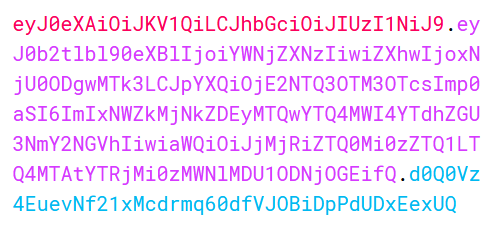
\includegraphics[width=110mm]{images/jwt_example.png}
    \caption{Exemplu de JWT folosit în Voting App}
\end{figure}

Într-un final, pentru a testa aplicația de backend, a fost folosită platforma Postman. Aceasta permite crearea de cereri HTTP și gruparea acestora într-un mod intuitiv. Au fost create cereri pentru toate Url-urile din aplicația de backend, fiind incluse și header-ele necesare.

\section{Baza de date}

\subsection{SQL}

Structured Query Language (SQL) este un limbaj de programare ce permite o interacțiune rapidă și eficientă din punct de vedere al timpului de execuție cu bazele de date. Acesta a fost dezvoltat de către inginerii de la IBM în anul 1974 și a rămas, încă de atunci, una dintre cele mai populare opțiuni atunci când vine vorba de dezvoltarea unei baze de date. Acest limbaj permite realizarea operațiilor de tip CRUD, fiind completat de o gamă variată de funcționalități precum: join-uri, indexări, operații matematice și nu numai.

\subsection{MySQL}

MySQL este un sistem open source de gestionare a bazelor de date relaționale, fiind creat de către Monty Widenius. Bazele de date relaționale stochează datele în tabele diferite, legate între ele prin chei de tip \enquote{foreign} \cite{what_is_mysql}. Pentru Voting App a fost folosit MySQL în scopul de a salva toate datele gestionate de către aplicația backend, astfel, fiind generate tabele, atât pentru modelele create cât și pentru cele \enquote{default}, necesare rulării Django și a librăriilor adăugate.

\begin{figure}[!h]
    \centering
    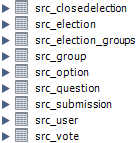
\includegraphics[width=45mm]{images/my_sql_example.png}
    \caption{Exemplu de tabele folosite pentru modelele din aplicația backend}
\end{figure}
\chapter{Utilizarea aplicației}

\section{Utilizator}
\subsection{Autentificarea}

Autentificarea reprezintă primul pas în utilizarea aplicației Voting App. Pentru a îmbunătății securitatea platformei, utilizatorilor nu le este permis să se înregistreze singuri, ei urmând să primească, atunci când le este creat contul de către un administrator, un mail pe adresa lor cu parola aferentă contului, parolă ce poate fi schimbată mai târziu, sau în cazul în care este uitată.

\begin{figure}[!ht]
    \centering
    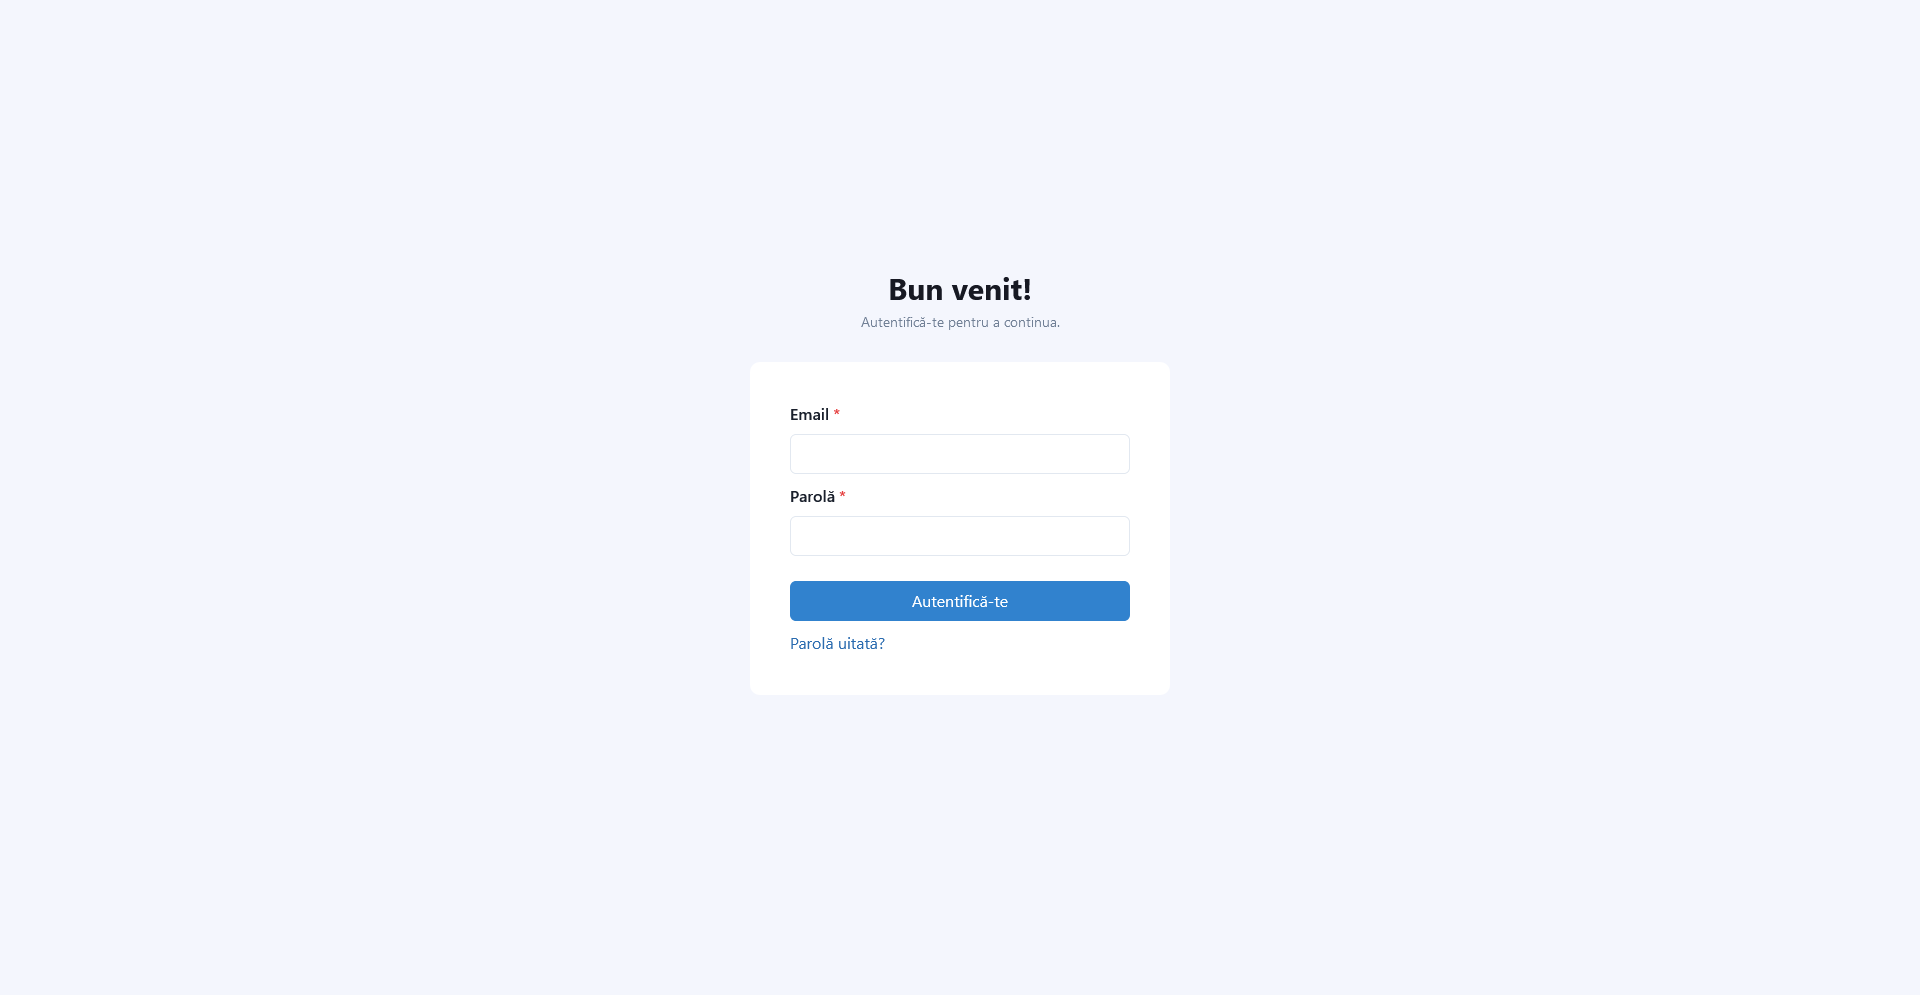
\includegraphics[width=145mm]{images/page_login.png}
    \caption{Captură a paginii de autentificare}
\end{figure}

\begin{figure}[!ht]
    \centering
    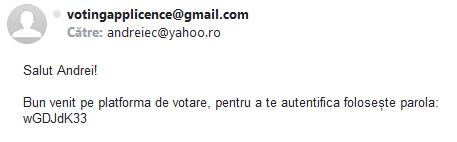
\includegraphics[width=115mm]{images/example_mail_register.png}
    \caption{Exemplu de mail primit atunci când este creat un cont nou}
\end{figure}

\subsection{Meniul principal}

Meniul principal reprezintă punctul de start al aplicației și locul în care se va desfășura cea mai mare parte a unui utilizator pe platformă. Acesta conține datele utilizatorului și ultimele procese electorale în care acesta a fost inclus. De asemenea, conținutul tuturor paginilor este înfășurat în componenta \enquote{Layout}. Pentru a oferi o experiență cât mai plăcută și mai rapidă, a fost realizat un design minimalist ce scoate în evidență punctele de interes.

\begin{figure}[!ht]
    \centering
    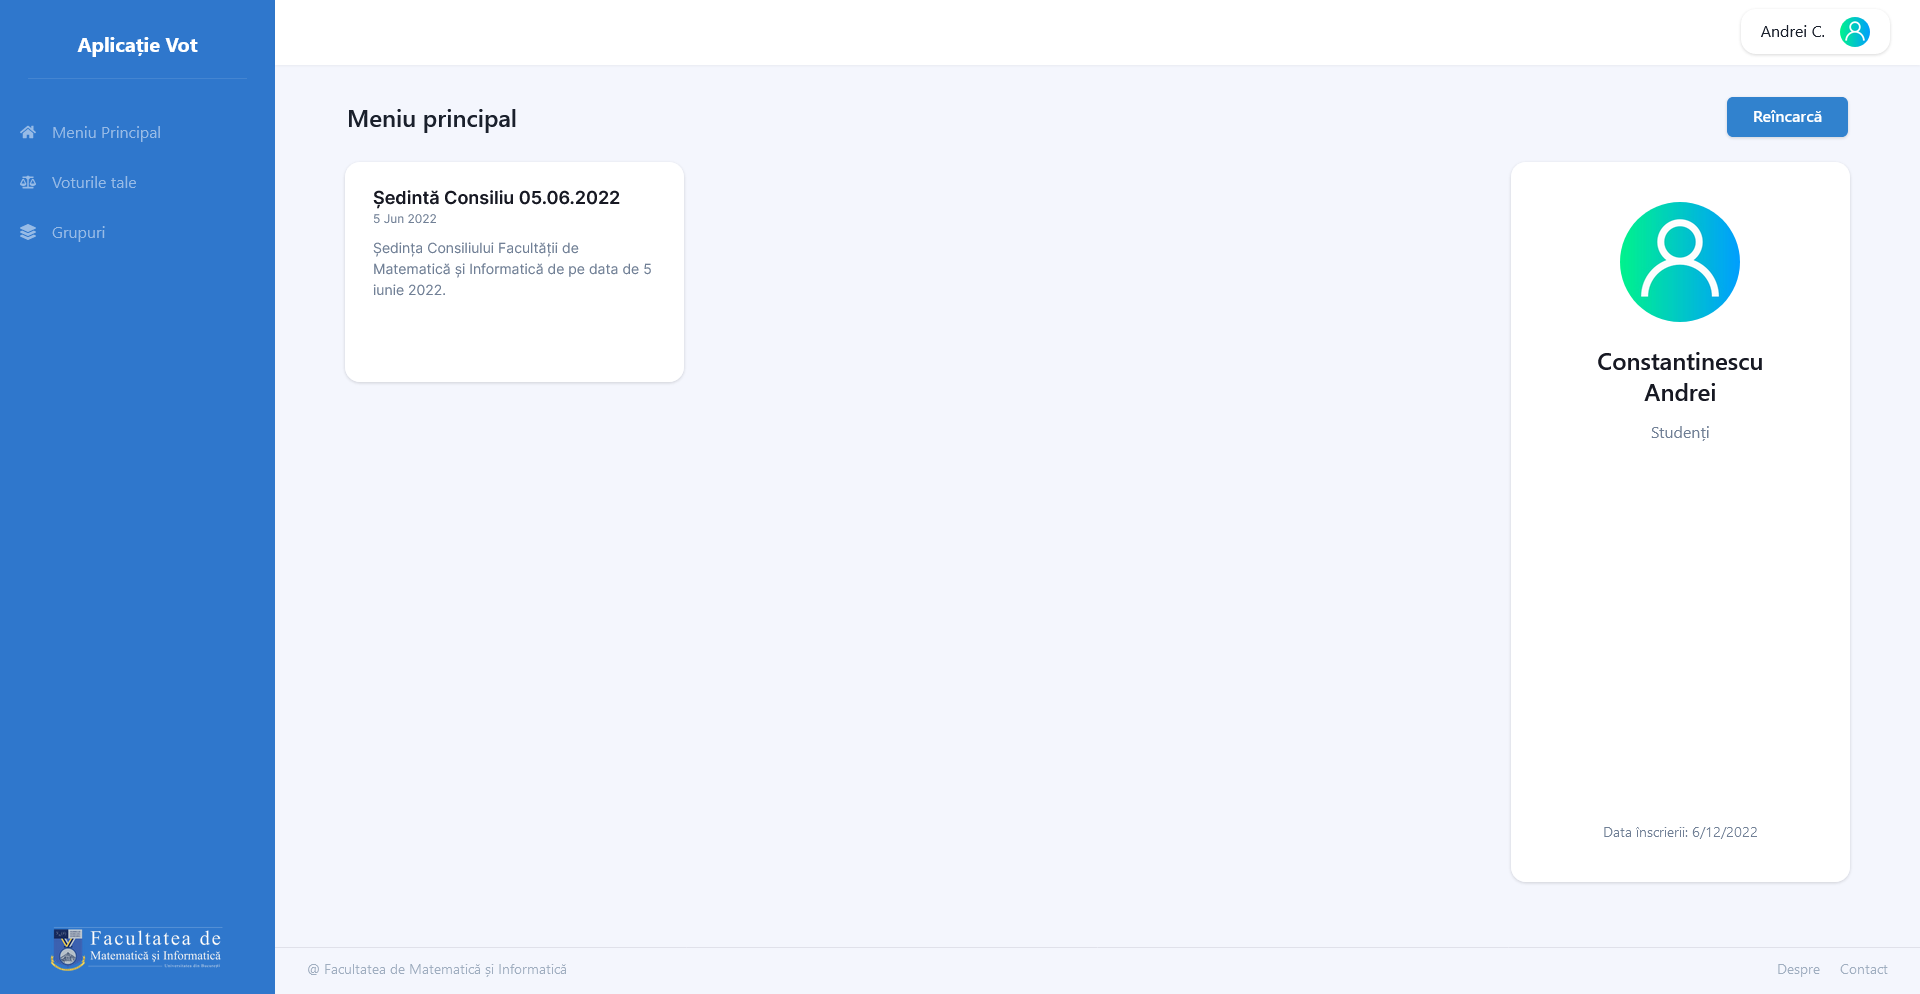
\includegraphics[width=145mm]{images/page_main.png}
    \caption{Captură a meniului principal}
\end{figure}

Componenta \enquote{Layout} conține, la rândul ei, alte patru componente: \enquote{Navbar}, \enquote{Sidebar}, \enquote{Titlebar} și \enquote{Footer}. În cazul în care utilizatorul este și administrator, componenta \enquote{Sidebar} va dispune de un buton suplimentar intitulat \enquote{Admin} ce va redirecționa utilizatorul către meniurile aferente.

\begin{figure}
\centering
\begin{subfigure}{.5\textwidth}
    \centering
    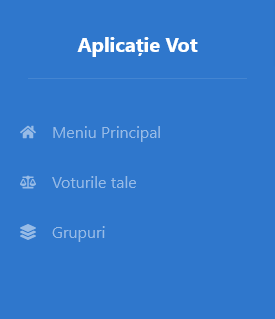
\includegraphics[width=45mm]{images/sidebar_normal.png}
\end{subfigure}%
\begin{subfigure}{.5\textwidth}
    \centering
    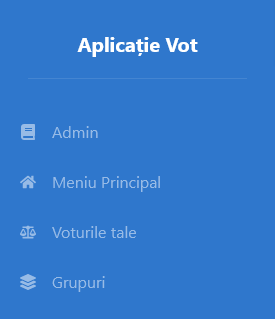
\includegraphics[width=45mm]{images/sidebar_admin.png}
\end{subfigure}
    \caption{Diferența componentei \enquote{Sidebar} între un utilizator și un administrator}
\end{figure}

\subsection{Pagini alternative}

Pe lângă meniul principal, utilizatorul mai are acces la câteva pagini:

\begin{itemize}
    \item \enquote{Voturile tale}. Aceasta conține totalitatea proceselor electorale la care utilizatorul a participat. Diferența dintre această pagina și meniul principal este lipsa cardului cu informațiile utilizatorului și prezența a absolut tuturor proceselor electorale, nu numai cele recente (prin recente se înțelege ultimele nouă procese electorale).
    \item \enquote{Grupuri}. Prezintă toate grupurile existente de pe platformă, astfel încât, în urma accesării unuia dintre grupuri, utilizatorul să primească detaliile aferente - nume, descriere, culoare și utilizatorii care fac parte din acel grup.
    \item \enquote{Setări}. Are o singură funcționalitate - conține un formular prin care utilizatorul își poate schimba parola contului.
\end{itemize}

\begin{figure}[!ht]
    \centering
    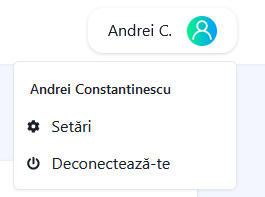
\includegraphics[width=65mm]{images/settings_button.png}
    \caption{Accesarea pagini \enquote{Setări} se realizează prin butonul din componenta \enquote{Navbar}}
\end{figure}

\subsection{Procesul de votare}

Atunci când un nou proces electoral este creat, un nou cartonaș ce conține numele și descrierea votului va apărea pe meniul principal, iar, pentru a accesa chestionarul de votare, este necesară doar o simplă apăsare pe cartonaș.

\begin{figure}[!ht]
    \centering
    
\includegraphics[width=95mm]{images/cartonas_vot.png}
    \caption{Exemplu de cartonaș de vot}
\end{figure}

Imediat după accesare, utilizatorul va primi buletinul de vot unde își poate exprima opțiunile. De asemenea, în Voting App este implementată validarea datelor astfel încât să fie respectate cerințele unei întrebări, de exemplu numărul maxim sau numărul minim de opțiuni necesare unei selecții multiple. Butonul de \enquote{submit} va fi activat doar când formularul este valid.

\begin{figure}[!ht]
    \centering
    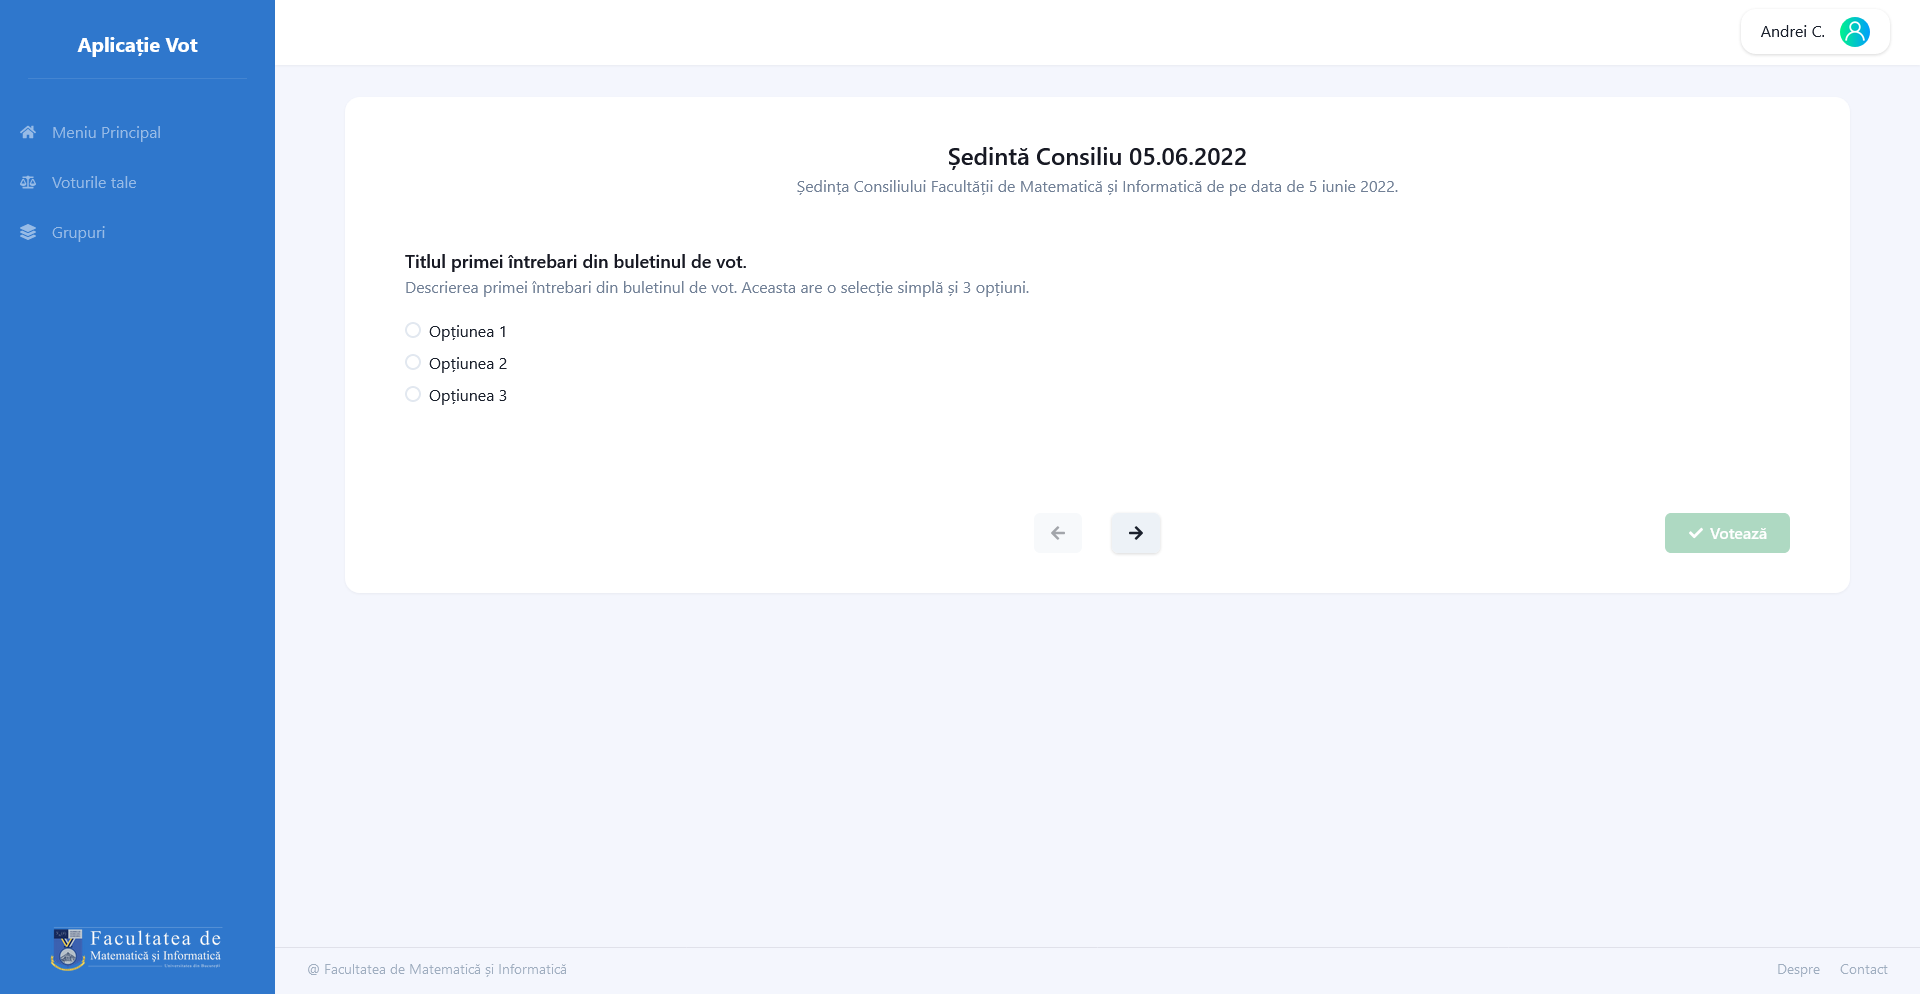
\includegraphics[width=145mm]{images/page_vote.png}
    \caption{Exemplu de buletin de vot, fiind prezentată prima întrebare din cele 2 date drept exemplu}
\end{figure}

\begin{figure}
\centering
\begin{subfigure}{.5\textwidth}
    \centering
    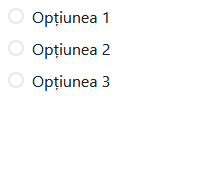
\includegraphics[width=45mm]{images/single_select.png}
\end{subfigure}%
\begin{subfigure}{.5\textwidth}
    \centering
    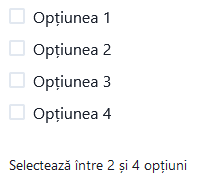
\includegraphics[width=45mm]{images/multiple_select.png}
\end{subfigure}
    \caption{Diferența între întrebările cu selecție simplă și cele cu selecție multiplă}
\end{figure}

În cadrul unui buletin de vot, utilizatorului îi pot fi adresate două tipuri de întrebări: cu selecție simplă, sau cu selecție multiplă. În cazul unei întrebări cu selecție simplă, utilizatorul poate alege numai una dintre opțiuni, pe când, în cazul unei întrebări cu selecție multiplă, utilizatorul poate alege mai multe opțiuni, fiind necesară încadrarea între un număr minim și un număr maxim de alegeri făcute.

Atunci când utilizatorul a completat toate chestionarele într-un mod corect, poate să își depună votul apăsând pe butonul \enquote{Votează}, unde va primi o notificare pe ecran pentru a confirma dacă este sigur de alegerea făcută. În urma confirmării și procesării de către aplicația de backend, acesta va fi redirecționat pe o pagină unde va apărea că votul lui a fost înregistrat. De asemenea, încercarea de a reaccesa formularul de vot va rezulta tot în afișarea mesajului de confirmare pentru a evita posibilitatea unei exprimări multiple a votului.

\begin{figure}[!ht]
    \centering
    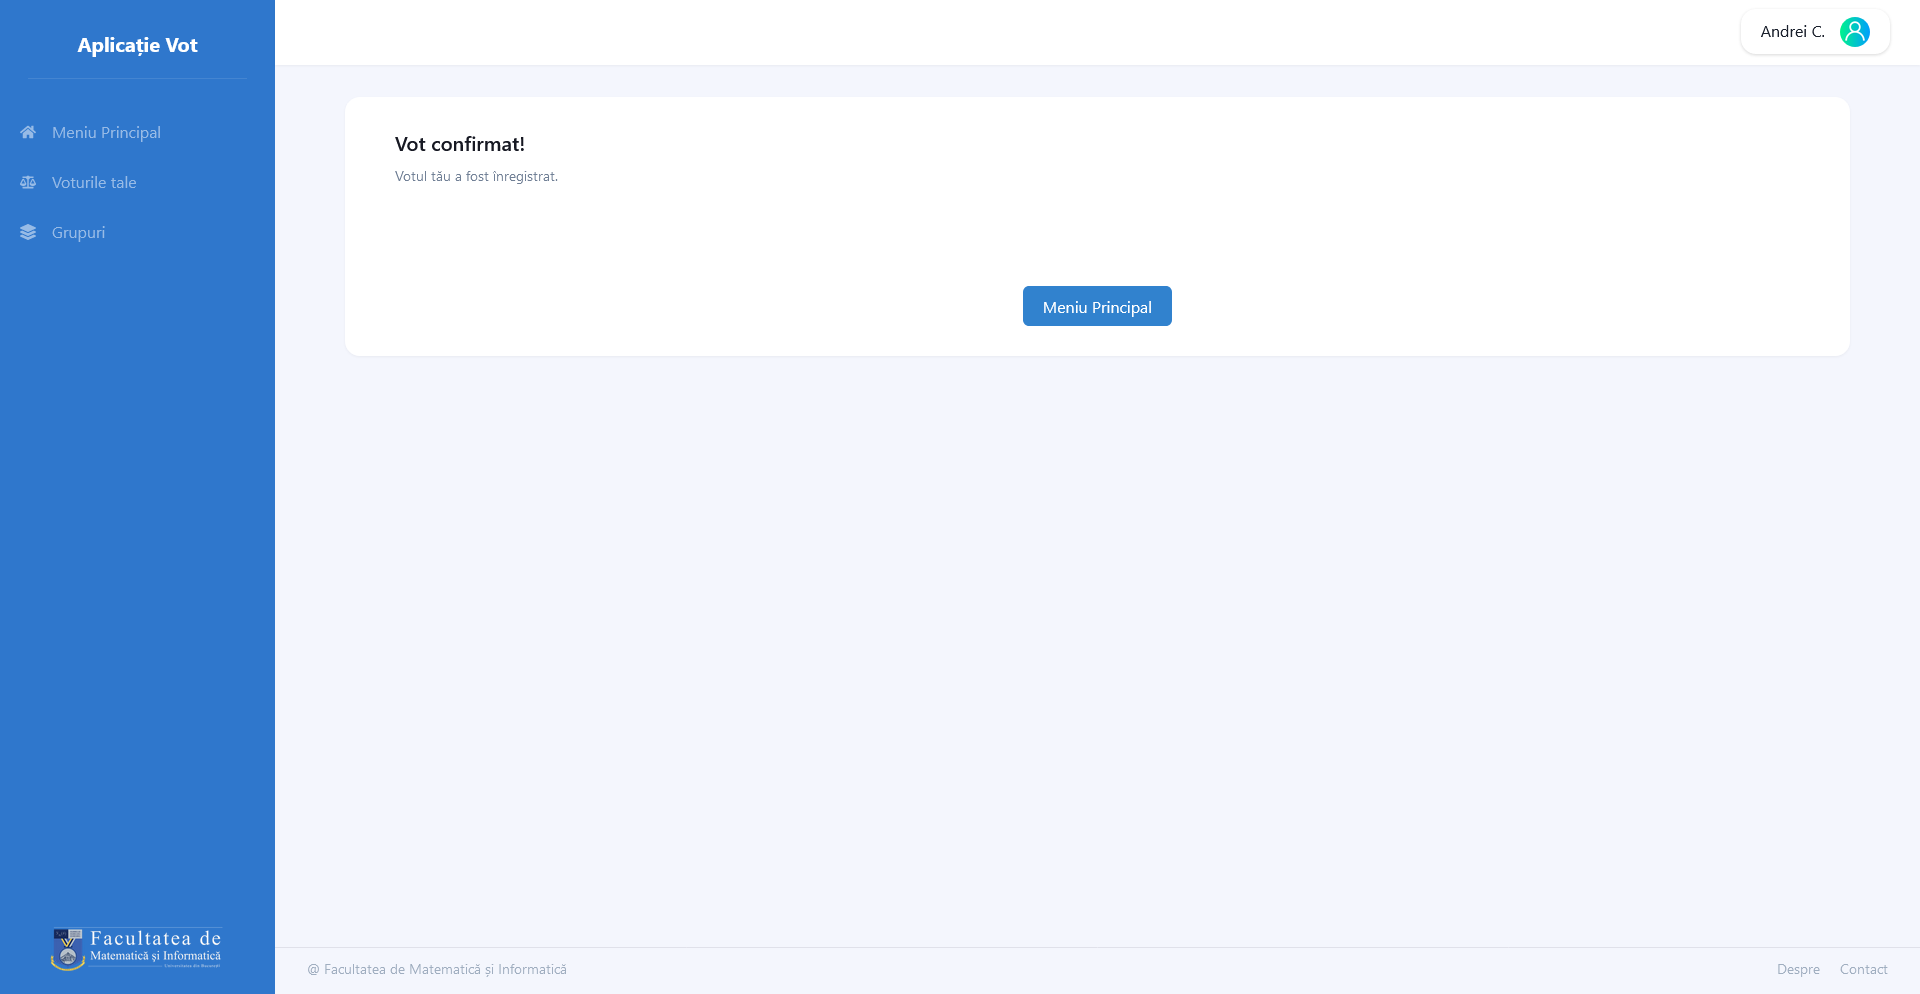
\includegraphics[width=145mm]{images/vote_confirmed.png}
    \caption{Captură a mesajului de confirmare}
\end{figure}

\subsection{Securitatea votului}

Deși HTTPS reprezintă un protocol securizat pentru transferul de date, aplicația Voting App adaugă un strat în plus de securitate atunci când vine vorba de încercarea înregistrării unui vot fals. Pentru a realiza acest lucru a fost implementată o funcție de \enquote{hash} ce are primește diverse date pentru a genera un cod de 256 de bits care este trimis spre aplicația de backend, odată cu finalizarea exprimării opțiunilor de vot, pentru a fi verificat. În cazul în care hash-ul nu este valid, votul depus nu o sa fie validat, astfel interceptând diverse încercări din afară de a falsifica voturi.

Funcția folosită pentru a genera hash-ul este SHA256, inventată în 2001 de către Agenția de Securitate Națională a Statelor Unite ale Americii și reprezintă, chiar și în ziua de azi, un standard în ceea ce înseamnă \enquote{hashing} \cite{what_is_hashing}. Deseori, acest algoritm este folosit pentru salvarea parolelor în bazele de date, astfel încât, în urma posibiltății unui atac cibernetic, atacatorii să nu aibă acces la parolele utilizatorilor, ci doar la hash-ul acestora.

\begin{code}
\begin{minted}[bgcolor=bg,frame=lines,framesep=2mm,fontsize=\footnotesize,baselinestretch=1]{js}
    // Preparing hash data
    const sent_on = new Date().toISOString();
    let hash = sha256(`${userSelector.id}.${params.id}.${sent_on}`);
\end{minted}
\captionof{figure}{Exemplu de cod pentru generarea hash-ului unui vot}
\label{code:hash-code}
\end{code}
\hfill

Securitatea algoritmului SHA256 este modelată de caracterul său ireversibil, dat fiind imposibilitatea realizării unui atac de tip \enquote{brute-force} într-un timp rezonabil, având la dispoziție nivelul tehnologic actual \cite{how_secure_sha}. În generarea unui hash, sunt utilizate atât funcții ireversibile, cât și de compresie, ce transformă datele de input. Un alt avantaj al folosirii acestui algoritm față de un altul este posibilitatea infimă de a întâmpina o coliziune - cazul în care două input-uri diferite rezultă în același output.

În aplicația Voting App, a fost folosit ca input al funcției SHA256 un string ce a rezultat din concatenarea identificatorului utilizatorului care și-a exprimat votul, identificatorului procesului electoral și data și ora exactă la care a fost depus votul, toate separate prin câte un punct. Rezultatul final va fi, întotdeauna, un șir de caractere de lungime 98.

\subsection{Schimbarea parolei}

Schimbarea parolei de către un utilizator se poate realiza în două moduri: prin formularul de la pagina setări, ce conține două câmpuri - unul pentru parola nouă și unul pentru confirmarea acesteia, sau prin formularul de \enquote{forgot password} prezent pe pagina de autentificare, în cazul uitării parolei.

Cel de al doilea formular implică trimiterea unui mail pe adresa utilizatorului. Acesta va conține un link către un formular de schimbare de parolă asemănător celui de la pagina "Setări". Ambele formulare necesită utilizatorului să introducă o parolă de minim opt caractere și care să conțină cel puțin o literă mare și un caracter special.

\begin{figure}[!ht]
    \centering
    
\includegraphics[width=135mm]{images/reset_pass_mail.png}
    \caption{Exemplu de mail pentru resetarea parolei}
\end{figure}

Mailurile sunt trimise folosind protocolul SMTP (Simple Mail Transfer Protocol) \cite{what_is_smtp}, integrat direct în framework-ul de backend. Textele mailurilor sunt generate dinamic, folosind datele utilizatorului care a făcut un request ce necesită trimiterea de mailuri.

De asemenea, este necesară crearea unei adrese de mail dedicate pentru a putea efectua transferul de mailuri și salvarea credențialelor acesteia în aplicația de backend. Pentru Voting App am folosit serviciul Gmail al Google, alături de funcționalitățile \enquote{two-factor authentification} și \enquote{app password} astfel încât trimiterea de mailuri să fie realizată direct, fără vreo altă aplicație terță.

\newpage

\section{Administrator}

\subsection{Meniul principal pentru administrator}

În urma autentificării cu un cont de administrator, utilizatorul va putea avea puteri sporite asupra aplicației, de exemplu să creeze și să șteargă conturi și grupuri, să creeze procese electorale și să le arhiveze. De asemenea, acesta decide când se va închide un proces electoral. Pentru a putea folosi toate aceste funcționalități, acesta dispune de un meniu principal care poate fi accesat din \enquote{Sidebar}, apăsând pe butonul \enquote{Admin}.

\begin{figure}[!ht]
    \centering
    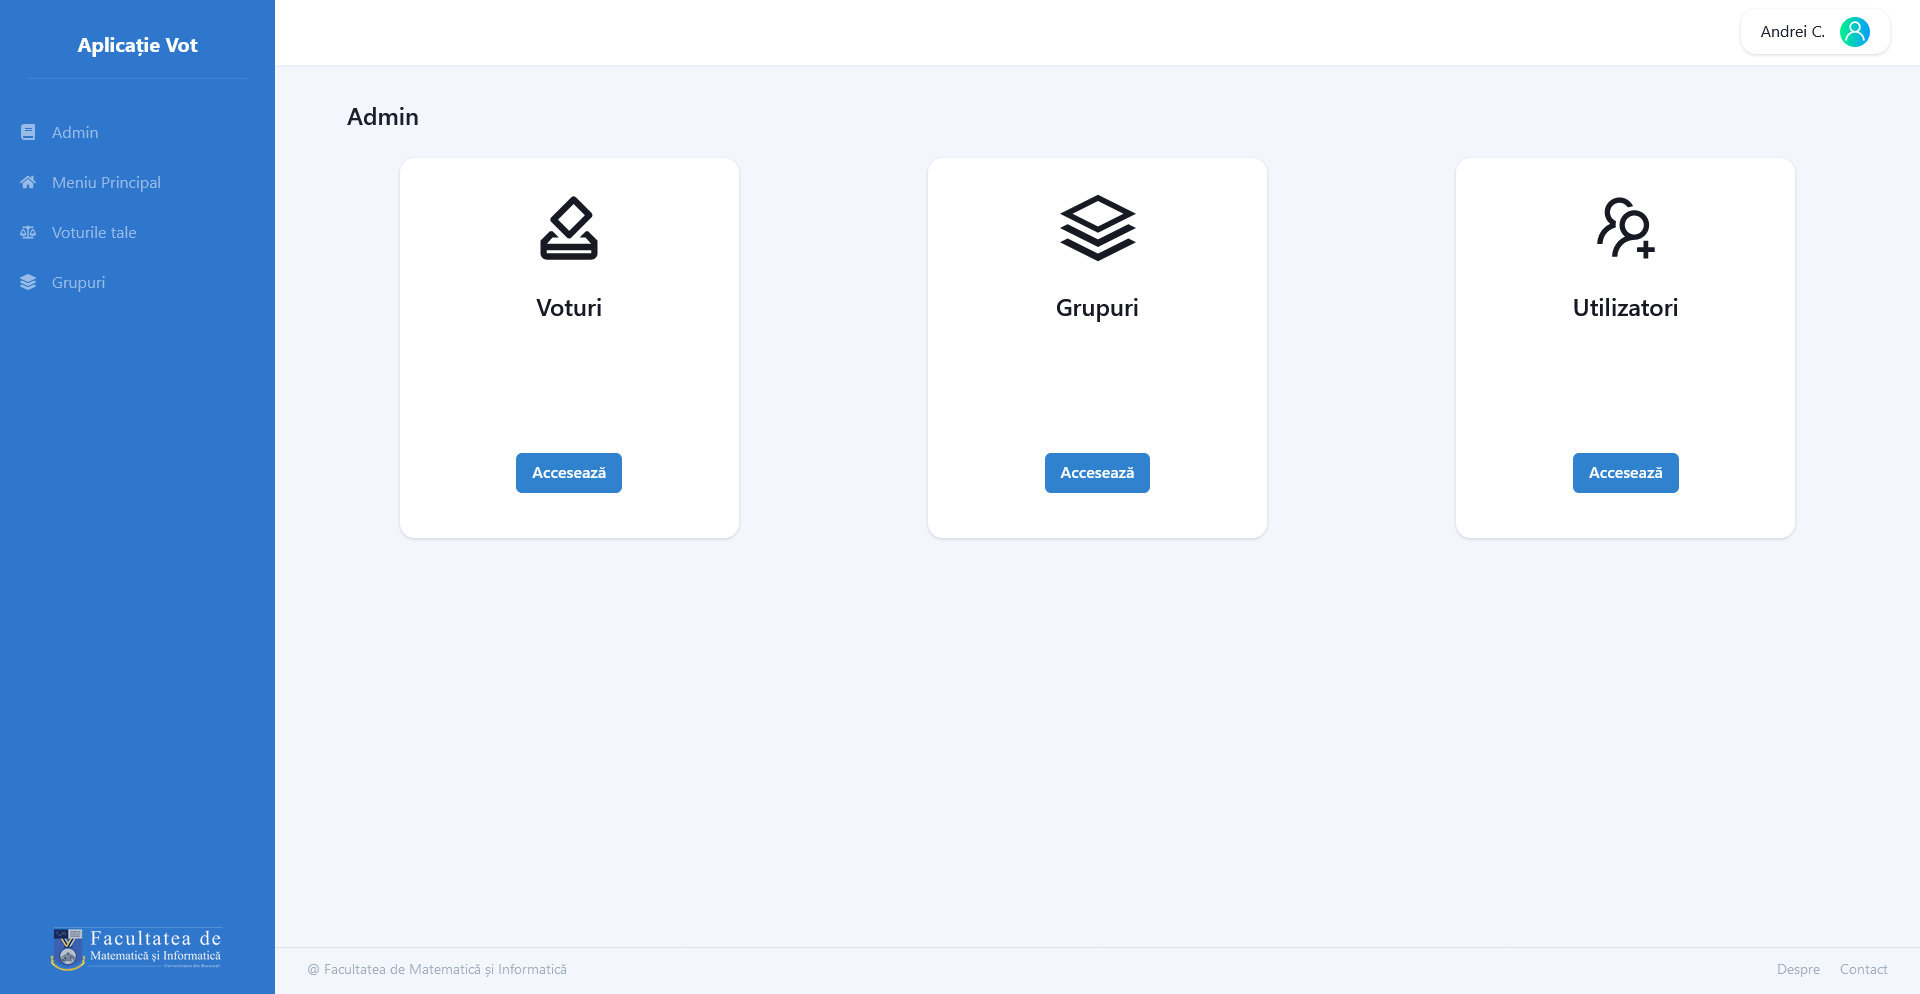
\includegraphics[width=135mm]{images/page_admin.png}
    \caption{Captură a meniului principal pentru administrator}
\end{figure}

Această pagină conține trei cartonașe ce permit administrarea rapidă și eficientă a platformei:

\begin{itemize}
    \item Cartonașul \enquote{Voturi}, conține formularul pentru a crea noi procese electorale și opțiunea de a le închide pe cele active.
    \item Cartonașul \enquote{Grupuri}, pentru a gestiona grupurile din platformă. Permite crearea, modificarea și ștergerea acestora.
    \item Cartonașul \enquote{Utilizatori}, folosit pentru a adăuga noi conturi pe platformă, a edita conturile active sau a le șterge pe cele inactive.
\end{itemize}

\newpage

\subsection{Crearea unui vot}

Primul cartonaș din meniul administratorului conține două tabele: cel pentru procesele electorale active și cel pentru procesele arhivate, accesat prin apăsarea butonului \enquote{Arhivă}. În dreptul fiecărui proces din listă se află un buton de \enquote{Detalii} ce va redirecționa administratorul în una din cele două opțiuni: în cazul unui proces electoral activ, pe pagina ce va arăta stadiul procesului, în direct, sau pe pagina de observare a rezultatului, în cazul unui proces încheiat și, implicit, arhivat. La baza tabelului din cadrul paginii de procese electorale active, se află butonul \enquote{Adaugă un vot}, menit pentru a redirecționa administratorul pe pagina ce conține formularul pentru crearea unui proces electoral.

Formularul de creare a unui vot reprezintă una dintre cele mai complexe funcționalități ale platformei, dat fiind caracterul lui dinamic. Pentru a crea un proces electoral, formularul a fost împărțit în trei segmente de bază:

\begin{itemize}
    \item Informații generale
    \item Grupuri
    \item Întrebări
\end{itemize}

Segmentul de informații generale conține două câmpuri: titlul buletinului de vot și descrierea acestuia. Aceste informații vor fi afișate pe toate paginile buletinului de vot.

Segmentul pentru grupuri este format dintr-o listă a tuturor grupurilor active pe platformă, unde administratorul poate selecta ce grupuri de utilizatori își vor exprima votul.

\begin{figure}[!ht]
    \centering
    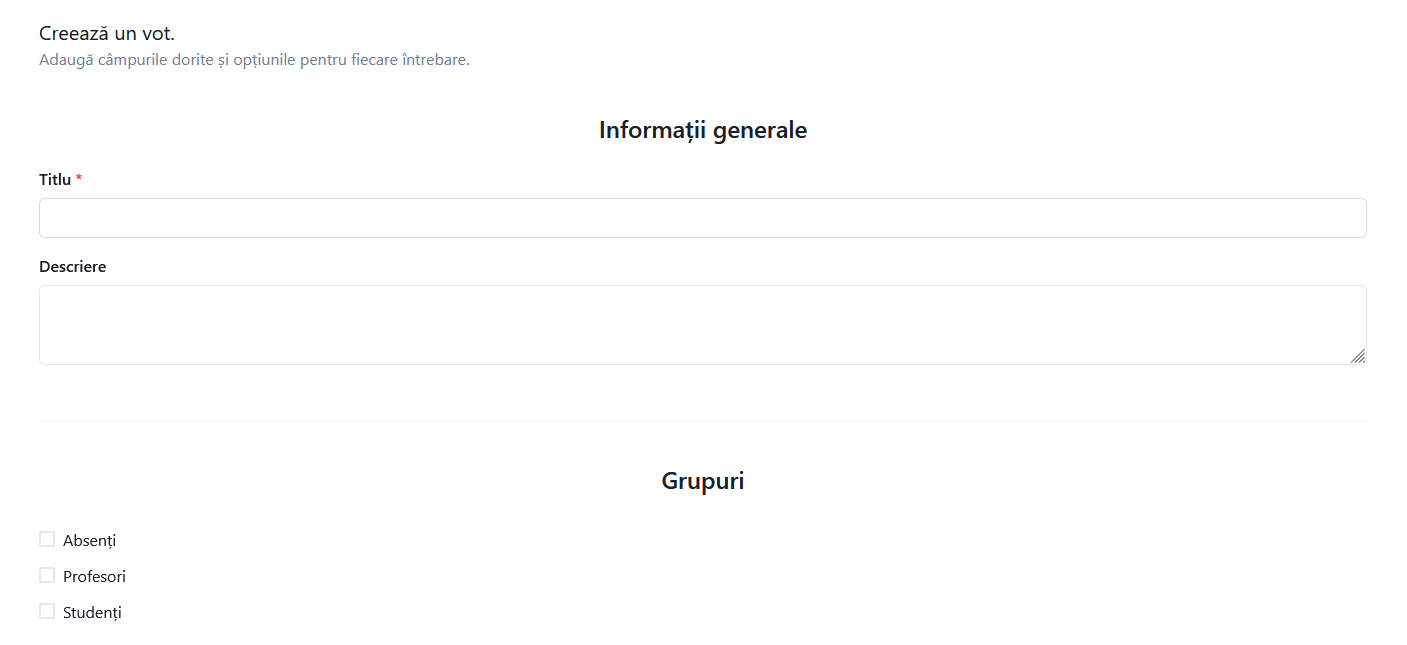
\includegraphics[width=145mm]{images/create_vote1.png}
    \caption{Segmentele \enquote{Informații generale} și \enquote{Grupuri}}
\end{figure}

Nu în ultimul rând, segmentul pentru întrebări conține o modalitate dinamică de generare a acestora și a opțiunilor aferente, similar funcționalității unui Google Form. Administratorul are de completat câmpurile pentru titlul și descrierea întrebării și de selectat tipul acesteia - selecție simplă sau selecție multiplă. În cazul în care administratorul decide să genereze o întrebare cu selecție multiplă acesta va fi nevoit să completeze câmpurile pentru selecții minime și selecții maxime. În cazul adăugării unei noi întrebări, acesta va apăsa butonul \enquote{Adaugă o întrebare}, iar în cazul ștergerii unei întrebări din listă, butonul \enquote{Șterge întrebarea}. Pentru fiecare întrebare, va fi nevoită generarea a cel puțin două opțiuni prin utilizarea câmpurilor aferente. Pentru a adăuga o opțiune, există butonul \enquote{Adaugă o opțiune}, iar pentru ștergere se va folosi butonul \enquote{X} din dreptul unei opțiuni.

\begin{figure}[!ht]
    \centering
    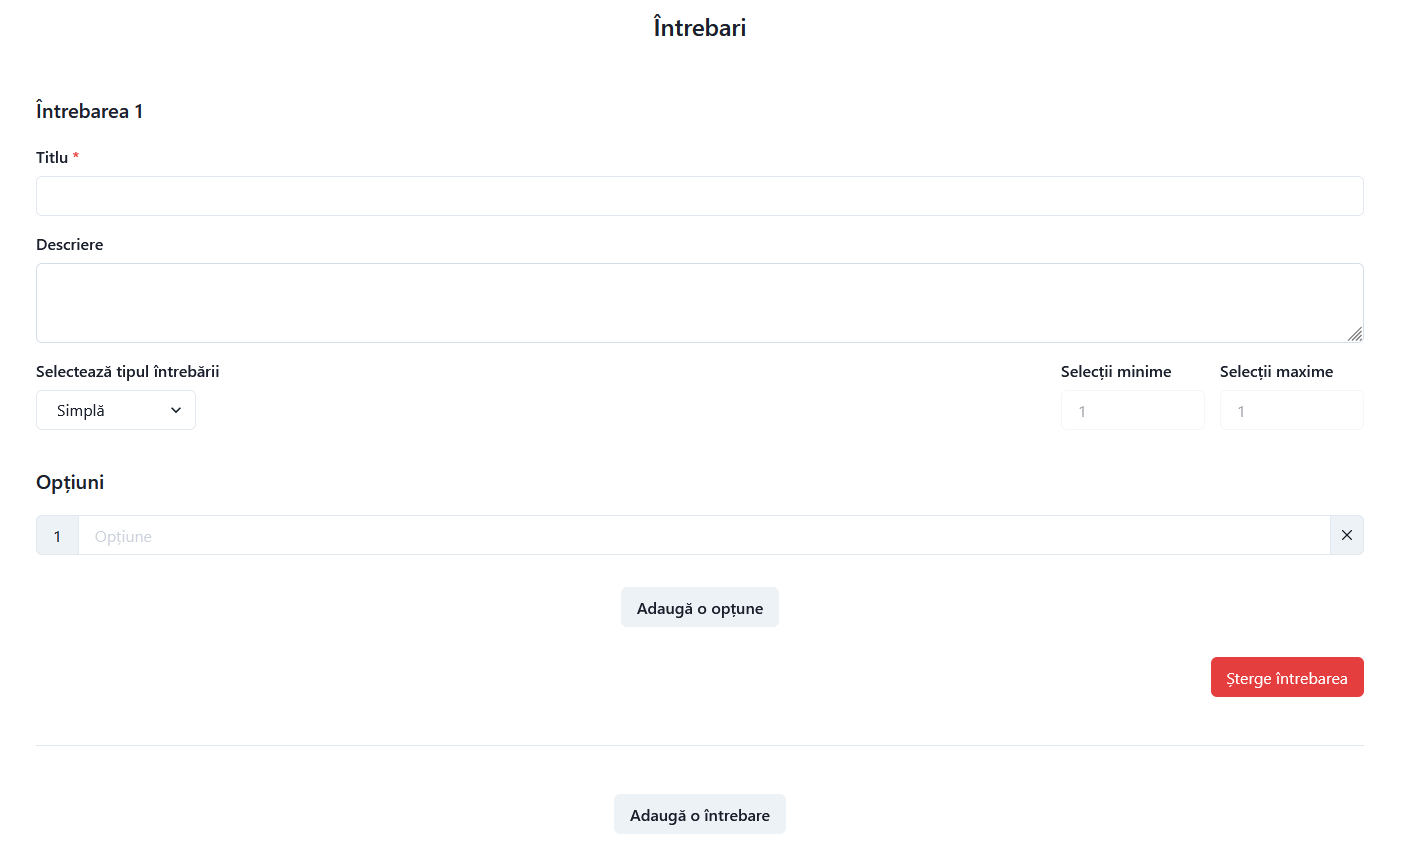
\includegraphics[width=135mm]{images/create_vote2.png}
    \caption{Segmentul \enquote{Întrebări}}
\end{figure}

Fiecare câmp din formular necesită validare, astfel, administratorul nu va putea genera un proces electoral dacă nu are toate câmpurile valide. Pentru fiecare câmp, chiar și cele create dinamic, va fi afișat un mesaj de avertizare în cazul în care acesta nu este valid.

Ultimul pas este reprezentat de apăsarea butonului \enquote{Finalizează} ce afișează administratorului un mesaj de confirmare. După confirmare, procesul electoral este început, iar utilizatorii își pot exprima votul.

\subsection{Încheierea unui proces electoral și observarea rezultatului}

Odată ce un proces electoral este creat, acesta va apărea în lista de procese electorale active din meniul "Voturi", unde, pentru fiecare proces în parte, există un buton \enquote{Detalii}, care va redirecționa administratorul către o pagină ce oferă statistici în direct asupra procesului electoral selectat. Pe această pagină apar informații despre stadiul actual, printre care: numărul total de votanți, numărul de votanți care și-au exprimat votul și lista acestora și butonul "Stop Vot". Atunci când expiră timpul de votare, sau administratorul decide să încheie votul, acesta va apăsa butonul pentru oprire și va fi redirecționat către pagina care va afișa rezultatul procesului electoral.

\begin{figure}[!ht]
    \centering
    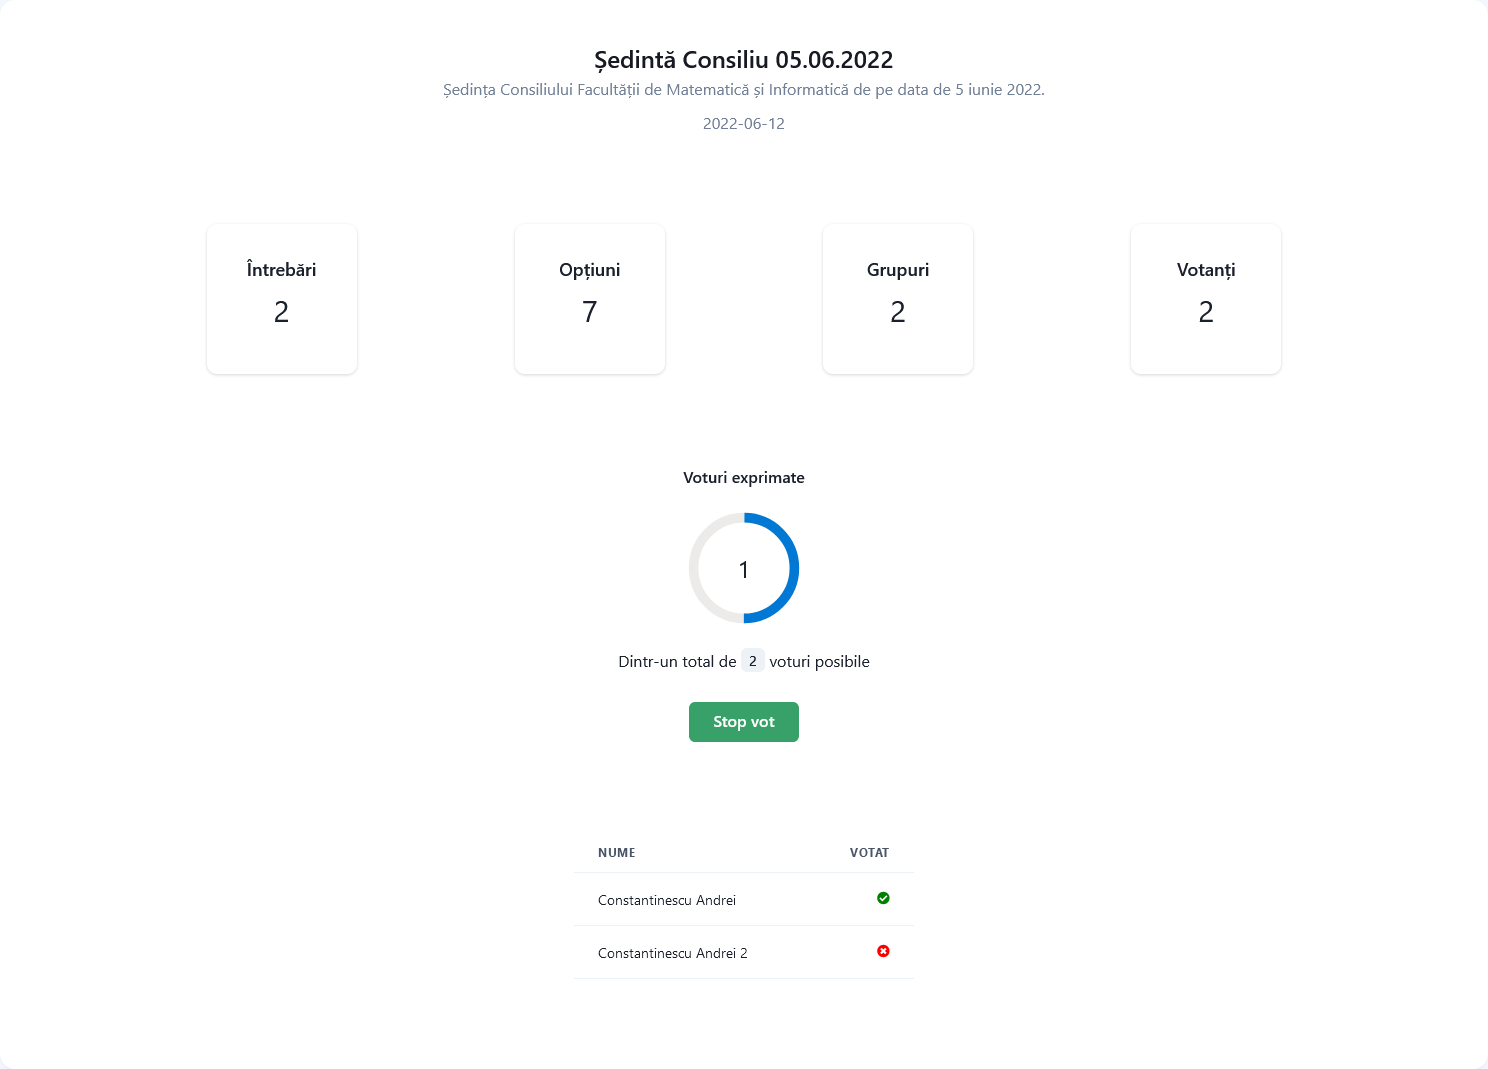
\includegraphics[width=135mm]{images/example_vote_details.png}
    \caption{Exemplu de detalii ale unui proces electoral}
\end{figure}

Pe pagina generată pentru observarea rezultatelor, vor fi afișate toate întrebările din buletinul de vot, fiecare cu opțiunile aferente și, în dreptul fiecărei dintre opțiuni, numărul de voturi exprimate în favoarea ei. În cazul în care o opțiune a unei întrebări reușește să strângă 50\% + 1 din voturi, aceasta va fi scoasă în evidență.

\begin{figure}[!ht]
    \centering
    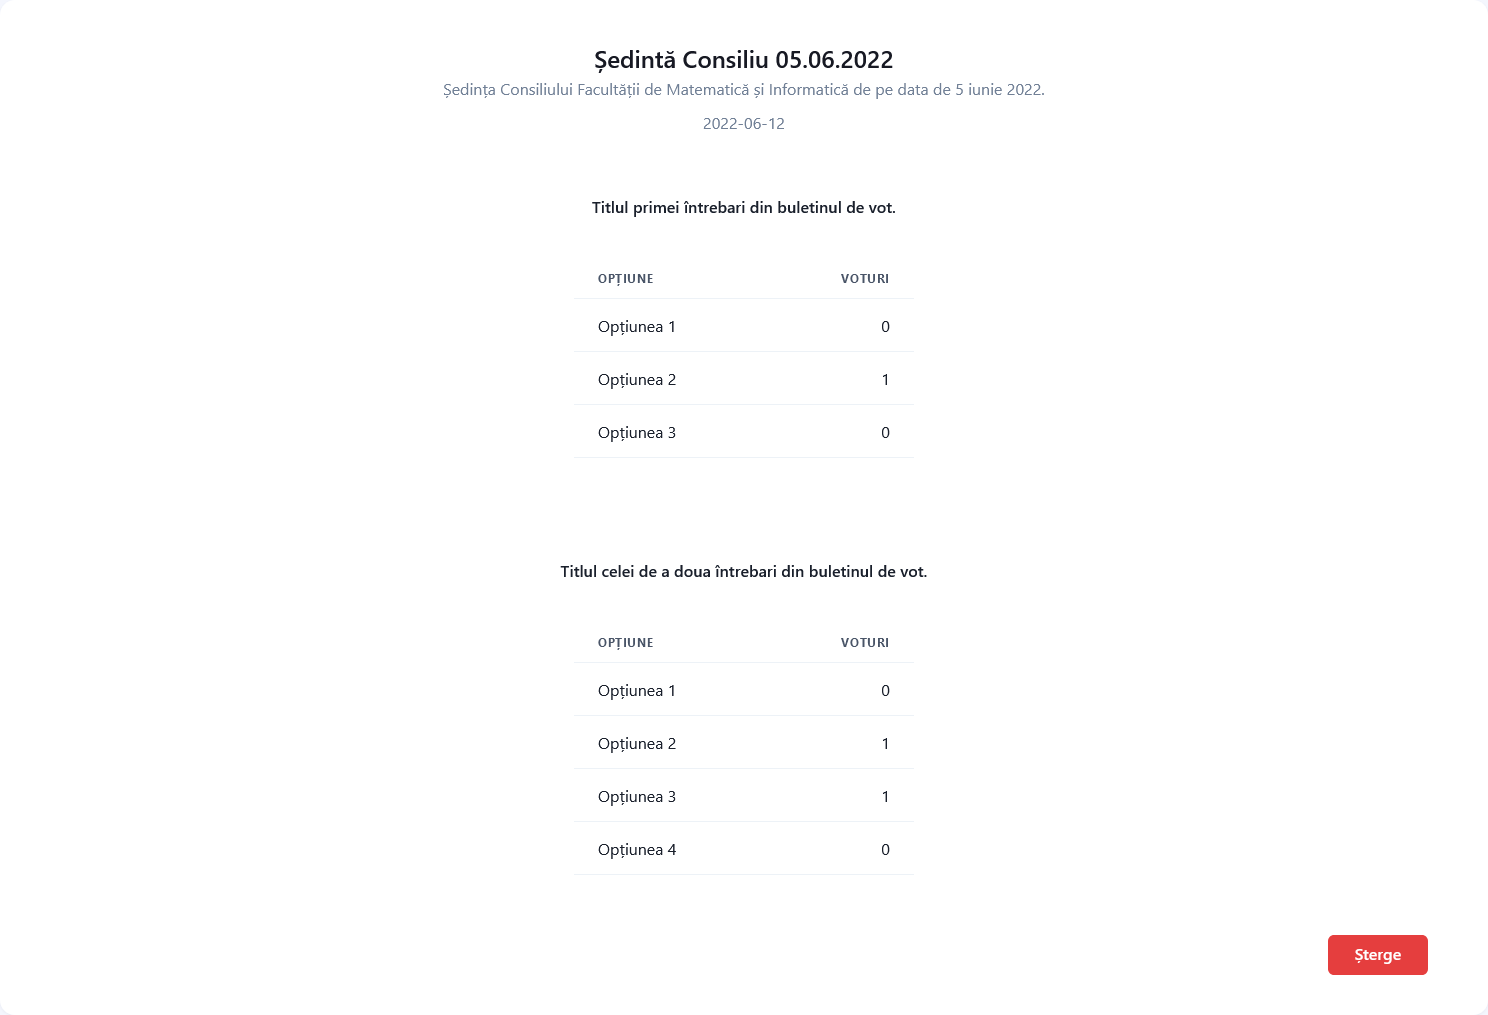
\includegraphics[width=135mm]{images/example_vote_results.png}
    \caption{Exemplu de rezultat al unui proces electoral încheiat}
\end{figure}

\newpage

\subsection{Operații de tip CRUD pe utilizatori și grupuri}

Următoarele două cartonașe din panoul de administrator sunt folosite pentru a accesa meniurile aferente operațiilor de creare, editare și ștergere atât a grupurilor, cât și a utilizatorilor. Ca funcționalitate, cele două se aseamănă, ambele conținând un formular ce se poate regăsi în două \enquote{state-uri} diferite - necompletat, în cazul creării unui cont de utilizator nou sau a unui grup nou, sau deja completat, caz în care valorile inițiale ale formularului vor conține datele aferente grupului sau utilizatorului ales. De asemenea, toate câmpurile din cele două formulare trebuie să fie valide pentru a putea continua.

\begin{figure}[!ht]
    \centering
    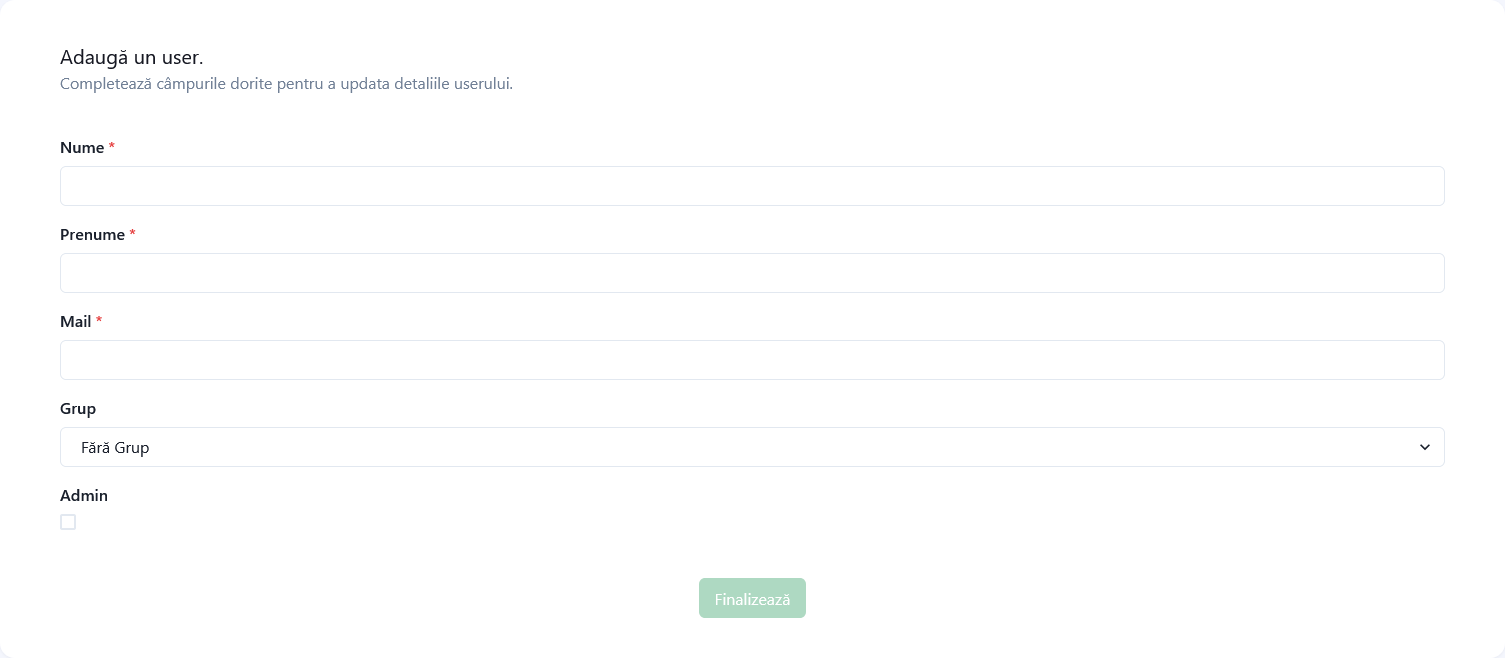
\includegraphics[width=140mm]{images/crud_user.png}
    \caption{Formularul pentru crearea unui cont de utilizator}
\end{figure}

\begin{figure}[!ht]
    \centering
    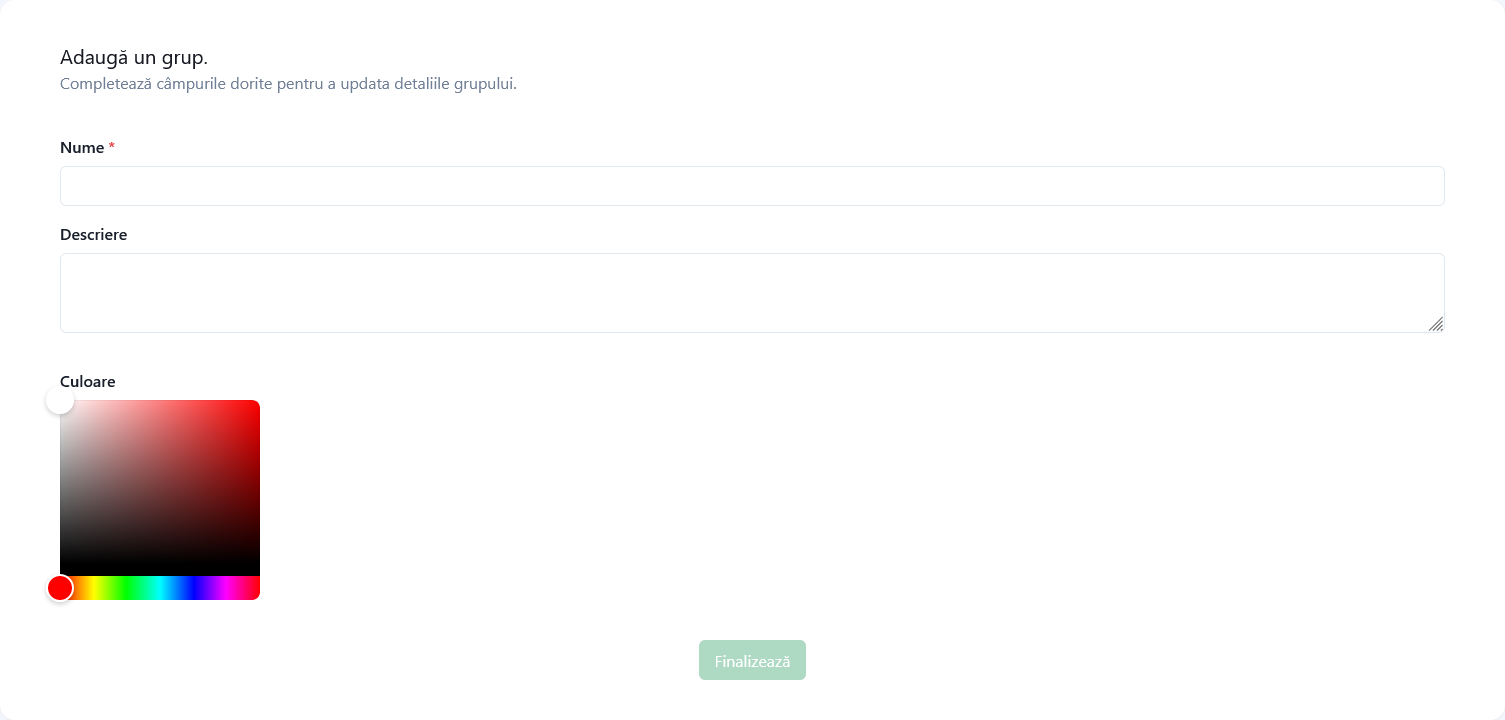
\includegraphics[width=140mm]{images/crud_group.png}
    \caption{Formularul pentru crearea unui grup}
\end{figure}

De asemenea, aplicația Voting App oferă și un strat de securitate în plus în ceea ce înseamnă modificarea datelor în timpul unui proces electoral activ. Platforma nu permite crearea, editarea, sau ștergerea atât a grupurilor, cât și a utilizatorilor  în timpul unui proces electoral deschis, dat fiind că acest lucru ar interveni în validitatea votului și implicit, în necesitatea atingerii cvorumului. În cazul în care administratorul dorește să efectueze schimbări asupra acestor modele, va trebui să închidă orice proces deschis, altfel va fi întâmpinat de o notificare cum că acțiunea pe care dorește să o facă este invalidă.

\newpage


\chapter{Concluzii}

În final, Aplicația Voting App a fost gândită cu scopul de a facilita un mediu cât mai eficient și mai sigur pentru exprimarea voturilor în cadrul Consiliului Facultății de Matematică și Informatică. Aceasta a apărut ca urmare a pandemiei de Covid-19, fapt ce a îngreunat toate activitățile ce se desfășurau într-un format fizic. Aplicația combină o suită de tehnologii variate, atât pe partea de client, cât și pe cea de server, aducând, pe deasupra, un design minimalist și ușor de interacționat. Dezvoltarea acestui proiect a reprezentat o posibilitate foarte bună de a înțelege și a aprofunda și mai mult cunoștințe în domeniul aplicațiilor web și al modului de utilizare a tehnologiilor implementate.

Desigur, există loc pentru îmbunătățiri și pentru implementat noi funcționalități. Printre acestea numărându-se: crearea în masă a conturilor de utilizator folosind documente de tip \enquote{.csv}, posibilitatea de a oferi mandat altui membru din consiliu pentru a vota în locul acestuia și nu numai. De asemenea, o altă versiune a acestei aplicații ar putea fi dezvoltată pentru a eficientiza procesul de alegere al studenților reprezentanți, dat fiind funcționalitatea de împărțire în grupuri pe care Voting App o are implementată.

\printbibliography[heading=bibintoc]



\end{document}